\documentclass[11pt]{article}
\usepackage{geometry} % see geometry.pdf on how to lay out the page. There's lots.
\usepackage{hyperref}
\usepackage{graphicx}
\usepackage{gensymb}
\usepackage[affil-it]{authblk}
\usepackage[toc,page]{appendix}
\usepackage{pifont}
\usepackage{amsmath}
\usepackage{amssymb}
\usepackage{relsize}
\usepackage{draftwatermark}
\usepackage[mathscr]{eucal}
\usepackage{amsmath, amssymb, graphics, setspace}
\usepackage{amsthm}
\usepackage[english]{babel}
\usepackage{listings}
\lstloadlanguages{Mathematica}
\usepackage{mathtools}
\DeclarePairedDelimiter{\norm}{\lVert}{\rVert}



\newcommand{\mathsym}[1]{{}}
\newcommand{\unicode}[1]{{}}

\newtheorem{exercise}{Exercise}
\newtheorem{theorem}{Theorem}
\newtheorem{corollary}{Corollary}
\newtheorem{conjecture}{Conjecture}
\newtheorem{observation}{Observation}



\SetWatermarkText{DRAFT}
\SetWatermarkScale{6}
\SetWatermarkLightness{0.95}

\DeclareMathOperator{\atantwo}{atan2}
\DeclareMathOperator{\sign}{sign}
\DeclareMathOperator{\sense}{sense}

% \geometry{letter} % or letter or a5paper or ... etc
% \geometry{landscape} % rotated page geometry

% See the ``Article customise'' template for come common customisations

\title{Calculating the Segmented Helix Formed by Repetitions of Identical Subunits and a Zoo of Platonic Helices}
\author{Robert L. Read
  \thanks{read.robert@gmail.com}
   email \href{mailto:read.robert@gmail.com}{read.robert@gmail.com}
}
\affil{Founder, Public Invention, a non-profit.}

\date{\today}

%%% BEGIN DOCUMENT
\begin{document}

\maketitle

\abstract{
Eric Lord has observed:
\begin{quote}
  In nature, helical structures arise when identical structural subunits combine sequentially, the orientational and translational relation between each unit
  and its predecessor remaining constant.\cite{lord2002helical}
\end{quote}
This paper proves Lord's observation as a consequence of screw theory.
Algorithm-like formulae for the segmented helix generated from the intrinsic properties of a stacked object and its
conjoining rule are given.
Standard results from screw theory\cite{wittenburg2016kinematics} and previous work for finding the axis of a helix from points\cite{kahn1989defining} are combined with
corollaries of Lord's observation to allow calculations of segmented helices from either transformation matrices or four known points.
The construction of these from the intrinsice properties of the rule for conjoining repeated subunits of arbitrary shape is provided.
allowin the complete parameters describing the unique
segmented helix generated by arbitrary stackings can be easily calculated.
Interactive software is provided which performs this computation for arbitray prisms along with 3D visualization.
This allows either the deduction of intrinsic properties of a repeated subunit from known properties of a segmented helix, as a chemist might
want to do, or the design of a segmented helix from known properties of a repeated subunit,
as a mechanical engineer or robotocist might want.
As a verification and demonstration, the software and paper compute, render, and catalog a ``zoo'' of all platonic helices,
such as Boerdijk-Coxeter tetrahelix and various
species of helices formed from dodecahedra, for example.
\tableofcontents


\section{Introduction}

During the Public Invention Mathathon of 2018\cite{read2019mathathon}, software was
created to view chains of regular tetrahedra joined face-to-face.
The participants noticed that whenever the rules for which face to add the next tetrahedron
to were periodic, the resulting
chain was always a helix.

Although unknown to us at that time, we now call Lord's Observation:
\begin{quote}
  In nature, helical structures arise when identical structural subunits combine sequentially, the orientational and translational relation between each unit
  and its predecessor remaining constant.\cite{lord2002helical}
\end{quote}
The purpose of this paper is to prove Lord's Observation and provide mathematical tools and software for studying arbitrary
segmented helices generated in this way.

Finding the properties of a segmented helix from four contiguous segments on the helix from screw theory\cite{abbasi2015review,wittenburg2016kinematics,wiki:screwaxis,kahn1989defining},
is explained and reformulated. An interactive, 3D rendering website written in JavaScript which allows both calculation and
interactive play and study. This allows
a structure or moleculde coincident to a segmented helix to be designed
by adjustments to the repeated object, or for the shape of
a repeated subunit to be inferred from the intrinsic properties of the
segmented helix.
Kahn's method \cite{kahn1989defining} is modified to cover some degenerate situations.

We exploit Lord's Observation to discover symmetry which allows us to compute the helix when subunits are joined face-to-face with
the same {\em twist.} Kahn was investigating proteins, which do not have faces, but geometric solids and other macroscopic solid objects do.
This concept can be generalized to a {\em joint face angle}, even if the
objects conjoined do not technically have flat faces.
This symmetry allows us compute the parameters of the segmente helix purely from
properties intrinsic to a single object and the joining rule.
Finally, as an important demonstration, these tools are used to produce
a catalog of all possible helices generated by vertex-matched face-to-face joints of the
Platonic solids, of which only the tetrahelix\cite{coxeter1985simplicial,sadler2013periodic,fuller1982synergetics,read2018transforming,pearce1990structure}
has been completely described to date.

\begin{figure}
     \centering
     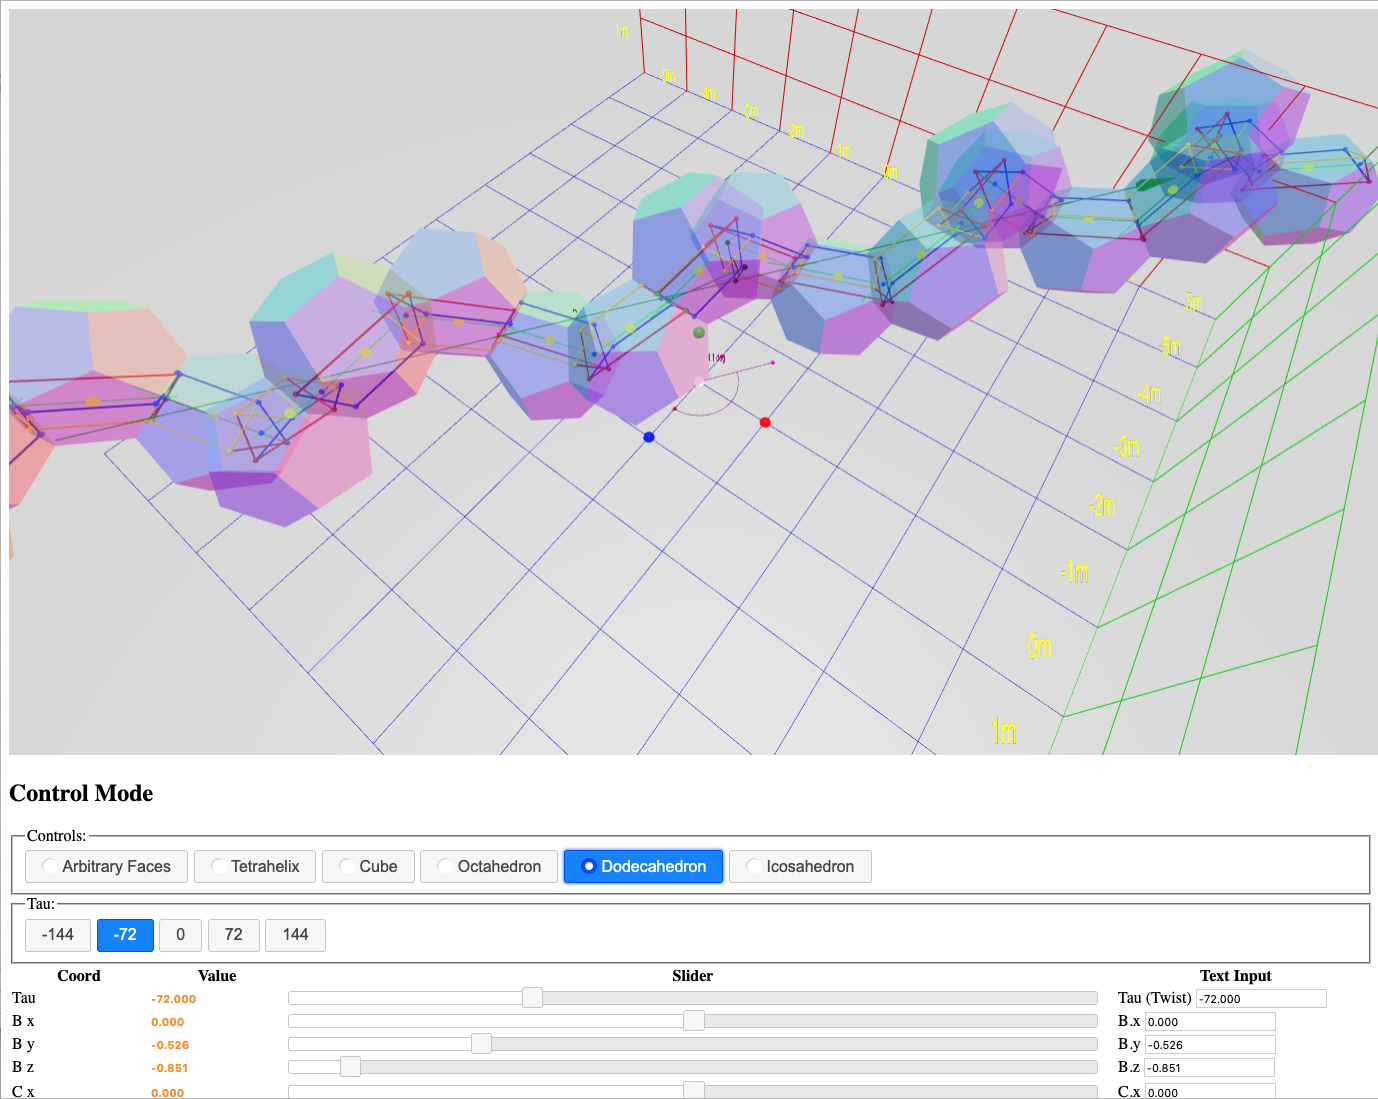
\includegraphics[width=0.80\textwidth]{figures/Dodecahedral.png}
     \caption{Example Segmented Helix Generated From the Dodecahedron}
  \label{fig:dodecahedron}
\end{figure}


\section{A Warm-up: Two Dimensions}

Considering the problem in two dimensions may be a valuable introduction.
Suppose that we consider a polygon that that as two edges, called $A$ and $B$, and that we define the length $L$ of the
polygon as the distance between the midpoints of these edges. Suppose that we are only allowed to join these
polygons by aligning $A$ of one polygon to $B$ of another polygon, with their midpoints coincident. Let us
further assume that we disallow inversions of the polygon.  Let us imagine that we have a
countable number of polygons $P_i$ indexed from $0$. Then what shapes can we make by chaining these
polygons together?

Each joint $J_i$ between polygons $P_i$ and $P_{i+1}$ will place the axes of at the same angle, $\theta$, since
our polygons do not change shape. Let us define $\theta$ to be positive
if we move anti-clockwise from $P_i$ to $P_{i+1}$ and negative if we move clockwise.
If $\theta = 0$, the joints will be collinear.

\begin{figure}
     \centering
     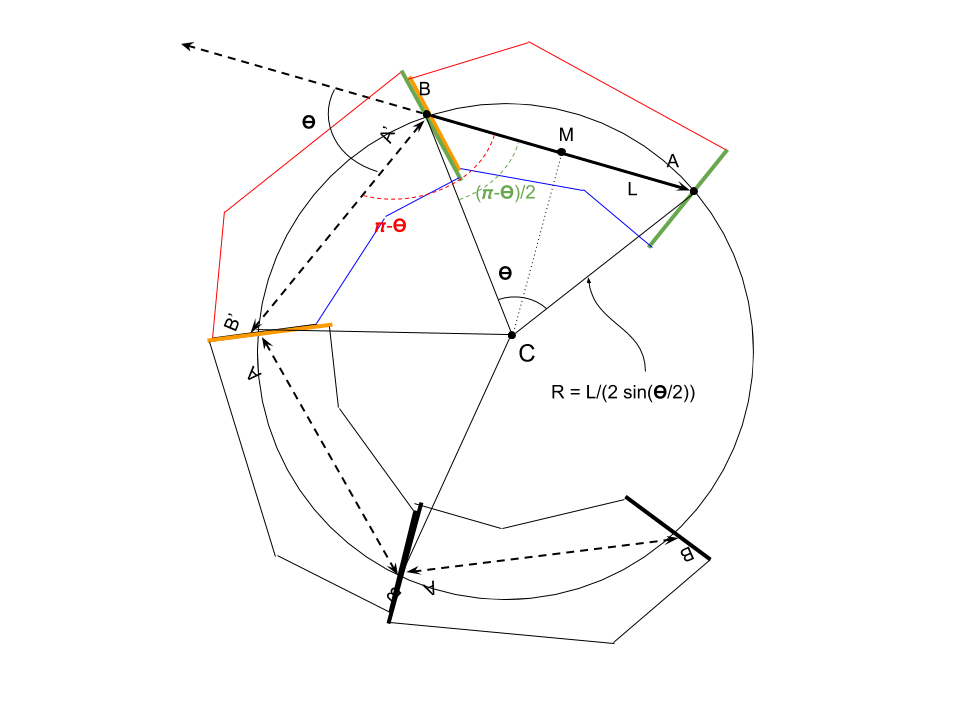
\includegraphics[width=0.80\textwidth]{figures/2DPolygonStacking.png}
     \caption{A 2D Analog of a Helix Generated by Repeated Subunits}
  \label{fig:prismdiagram}
\end{figure}

If $\theta \neq 0$, it seems they polygon joints will always lie on a circle. A proof of this
is that each polygon has associated with it an isosceles triangle $A,B,C$, where $\angle CBA = \angle CAB = \theta/2$,
and $\angle ACB = (\pi - \theta)$. $AC$ and $BC$ are not necessarily aligned with an edge of the polygon.
The length $AB$ is $L$, and the lengths $AC$ and $BC$ are
$(L/2) / \sin{(\pi - \theta)/2}$. In any chain of polygons, these triangles all meet at point $C$, and there all
joints are on the circle centered at $C$ with radius $\frac{L}{2 \sin{\frac{\theta}{2}}}$.


\label{sec:2d}

\section{The Segmented Helix}

An analogous result holds in three dimensions.

In this section we consider a helix evaluated only at regular points.

Following the Wikipedia article \url{https://en.wikipedia.org/wiki/Helix}, we set up a helix parametrically.
\begin{align*}
    P_x(t) &= r \sin{t}  \\
    P_y(t) &= r \cos{t} \\
   P_z(t) &= b t
\end{align*}
Such a helix has a radius of $r$ and slope (if $r \neq 0$) of $b/r$.
The pitch of helix, the change in $t$ needed to make one complete revoluion, is $2\pi b$.
Note that a helix may be degenerate in two ways.
If $r = 0$, these equations become a line. If $b = 0$, these equations describe a circle in the $xy$-plane.
If $r = 0$ and $b = 0$, the figure is a point.

Such helices are continuous, but we are investigating stacks of discrete objects. We in fact wish to derive
the parameters for a continuous helix from such discrete objects which constrain discrete points, so we wish
to study a helix evaluated at integral points. We call such an object a {\em segmented helix}.
A segmented helix may be thought of as function that given an integer gives back a point in three space.
\begin{align*}
    P_x(n) &= r \sin{n \theta}  \\
    P_y(n) &= r \cos{n \theta} \\
   P_z(n) &= n d
\end{align*}

$d$ is the distance or {\em travel} along the axis between adjacent joints. In this canoncial representation this is
the $z$-axis.
$\theta$ is the rotation around the $z$-axis
between adjacent points.
$r$ is the radius of the segmented helix.
Note that if $\theta = \pi$, we have a third form of degeneracy (to the human eye) of a segmented helix
which is a zig-zag contained completely within a single plane.

If we think of the segmented helix as describing a polyline in 3-space, we would like to investigate
the properties of that polyline. If we consider only the intrinsic shape of the segmented helix, there are three degrees
of freedom: $r,d,\theta$. We call these the {\em intrinsic} propertiers of the segmented helix.

A segemented helix located in space is completely determined by these parameters, a vector describing the axis
of the helix, and the position of any one joint.

Because the segmented helix is a discrete structure, we reframe the concept of {\em pitch} as {\em sidedness $s$}: how many segments (sides)
make a complete rotation?

\begin{itemize}
\item $L$ is the distance between any two adjacent points.
  \item $\theta$ rotation about the axis between two joints.
  \item $c$ is the length of a chord formed by the projection of the segment between two points projected along the axis of the segmented helix.
\item $d$ is the distance along the axis of the helix between any two joints.
\item $\phi$ is the angle between any vector between two adjacent joints and the axis of the helix. In physical screws used in mechanical engineering, this is analogous to the {\em helix angle} \cite{wiki:helixangle}.
  \item $p$ is the pitch of the helix, the distance travelled in one complete rotation.
  \item $s$ is the number of segments in a complete rotation (in general not rational.)
  \end{itemize}
These quantities are related:
\begin{align}
    c &= 2r\sin{\frac{\theta}{2}} \\
    L^2 &= c^2+d^2  \\
    \arctan{\frac{c}{d}}  &= \phi \\
    s &= \frac{2 \pi}{\theta} \\
    d &= L \cos{\phi} \\
    p &= d s \\
\end{align}

Measuring $\phi$ requires us to decide on the sign of the direction of the axis, which is aribtrary and not based on the
physical shape.

Any point on on the segmented helix has a closest point on the axis of the helix. In particular, we will call the points closest to the
joints {\em joint axis points}. Then $d$ is the distance along the axis between consecutive joint axis points.

We seek to relate these properties to properties intrinsic to the joint or interface between
two segments or objects in the segmented helix. If given an object, the length between the joints $L$ is intrinsic.

\label{sec:SegmentedHelix}

\section{The Intrinsic Properties of Periodic Chains of Solids}

If we have chains of repeated 3D units conjoined identically, they generate a segmented helix coincident on their joints.
Although fairly obvious from Chasles' Theorem, we have not found this stated in writing elsewhere, so we call this Lord's Observation:

\begin{observation}[Lord's Observation]
  “In nature, helical structures arise when identical structural subunits combine sequentially, the orientational and translational relation between each unit and its predecessor remaining constant.”\cite{lord2002helical}
\end{observation}
Lord's Observation may perhaps be clarified that in fact identical objects conjoined via a rule
produce periodic chains of objects that are uniformly intersected by segmented helices and that they may be degenerate in one of
three ways that we might not strike us as a helix if we are not seeking them:
\begin{enumerate}
\item The segments may form a straight line. (For example, see Figure \ref{fig:pearlshaft}).
\item The segments may be planar about a center, forming a polygon or ring. (For example, see Figure \ref{fig:thewheel}).
\item The segments may form a planar saw-tooth or zig-zag pattern of indefinite extent (For example, see Figure \ref{fig:planarzigzag}).
\end{enumerate}

\begin{figure}
     \centering
     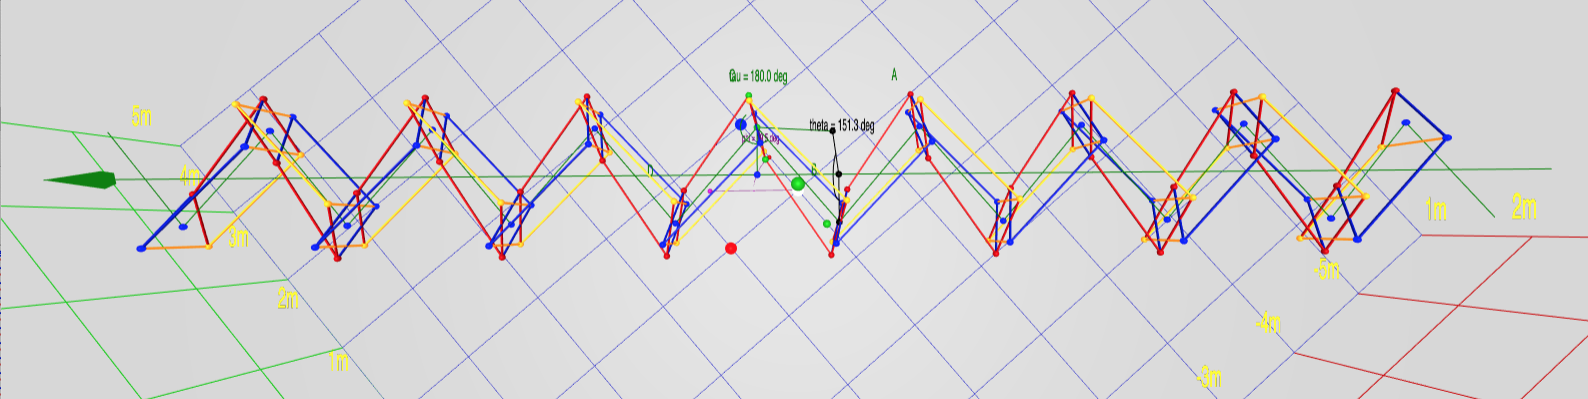
\includegraphics[width=0.80\textwidth]{figures/PlanarZigZag.png}
     \caption{A Planar Zig-Zag}
  \label{fig:planarzigzag}
\end{figure}

There are two complementary ways of learning about such segmented helices.
In one approach, we may have knowledge of the segmented helix, and
wish to learn about the subunits and the rule with which the subunits are combined.
For example, we may have microscopic objects such as proteins
or atoms, and we know from crystallography something about the positioning of these objects, without
knowing ahead of time the angles at which these objects would combine in their natural environment.
In this case, we use a variant of a linear algebra method\cite{kahn1989defining} for determining the radius, travel, and twist
of the segmented helix (these terms will be defined precisely below.)

In the other approach, we may know {\it a priori} exactly the
relevant properties of the objects and the rule which which they combine, and we seek to compactly describe the segmented helix they create.
For example, a mathematician may consider a chain of dodecahedra, or a woodworker may cut identical blocks of maple wood,
which are to be glued together face-to-face. In these cases everything about the objects and the rules for conjoining
is known before the first two objects are glued together. We call this the {\em joint face normal method}, because
it can be simulated by joining two flat faces together with a specified twist, even if the objects in question
do not actually have a physical face (such as molecules).

In both cases, we would like to understand how a change in a face normal or a twist affects the parameters
of the segmented helix,
and, conversely, we would like to be able to choose the construction of the subunits to achieve a particular segmented helix.

In engineering, sometimes the term {\em special helix}\cite{gu2012research} is use for helical curves on non-cylindrical surfaces. This paper use the term {\em helix} only in the sense of {\em cylindrical helix}.

\section{Periodic Chains Produce Segmented Helices}

A periodic chain is in fact a simple object which demonstrates tremendous symmetry.
Before using this symmetry in the construction of the segmented helix corresponding to a periodic chain, we
prove that such a segmented helix indeed exists.

\begin{theorem}[Segmented Helix]
  Consider $N$ identical objects which each have two points, $A$ and $B$, called {\em joints},
  and a vector $U$ not collinear with $A$ and $B$. Call
  $\overline{AB}$ the {\em axis} of this object.
  Consider the frame of reference for this object to have
  its axis on the $z$-axis with $B$ in the positive direction, the
  midpoint of the at the origin, and the up-vector pointing in the positive $y$ direction.

  Consider any rule that conjoins $A$ of object $i+1$ to $B$ such that
  from the frame of reference of $i$, the object $i+1$ and anything rigidly
  attached to it is always in the same position in the frame of reference for $i$.
  Informally, $i+1$ ``looks the same'' to $i$, no matter what $i$ we choose, $i < N$.
  Call a chain of $N$ identical rigid objects conjoined via a rule that
  conjoins $A$ to $B$ in such a way that every vector
  of $B$ is always in the same position relative to a frame of reference
  constructed from $A$ a {\em periodic chain.}

  Any periodic chain of three or more objects has a unique segmented helix who
  whose segments correspond
  to the axes of these objects.
\end{theorem}

\begin{proof}
  We will proceed by induction.

  Base Case ($k == 3$):

  Take an object $AB$. By Chasles' theorem\cite{wiki:chasles}
    there is a screw axis $S$, a set of rotations,  and a transposition $d$ which moves the first object to
    position where the second object $BC$ is. Take one of the rotation angles of smallest value.
    Construct the points $A'$, $B'$ and $C'$ as the closest points
  to $A,B$ and $C$ on this axis. These points are collinear by construction.

  Now add the object $CD$ to object $BC$ by our the rule of periodic chains. Consider the points
  $B'$ and $C'$ from $A$'s frame of reference. Let $d = \| \overline C' - \overline B' \|$.
  Construct the point $D'$ on our screw axis as the point closest to $D$ on that line.

  Now because $C'D'$ in $BC$'s frame or reference must look like $B'C'$ in $A$'s frame of reference,
  must look like $B'C'$, the distance $\| \overline D' - \overline C' \| = d$.
  From $A$'s frame of reference, $A'B'C'$ are collinear, the points $B'C'D'$ must be collinear in
  $B$'s frame of reference.

  In any frame of reference, if $A'B'C'$ are collinear and $B'C'D'$ are collinear, then $A'B'C'D'$
  are collinear.

  Now, looking backward from $CD$ towards $A$, the distance $A'B'$ must be the same as the
  distance $B'C'$ so as to not violate our rule. So $d = \| A'B' \| = \| B'C' \| = \| C'D'\|$.
  Similarly because by construction $r = \| B B' \| = \| C C' \|$, and $AA'$ is a rigid
  transformation of $BB'$, so $r = \| A A' \|$. By symmetry, $r = \| D D' \|$.
  Compute $\theta$ as the rotation about $S$ that takes $B B'$ into $C C'$. By our rule
  of attachment, $\theta$ also takes $C C'$ into $D D'$ and $A A'$ into $B B'$.

  Now construct a segmented helix, the radius $r$, distance,
  and angle $\theta$. This segmented helix can be positioned coincident with $S$ so
  that $H_0 = A$. Then $H_1=B$, $H_2=C$, and $H_3=D$.

  Therefore, for the base case of three objects, there is a segmented helix whose
  segments coincide with the axes of the objects.


  Inductive Case ($k+1$):
  Assume there is a segmented helix coinciding with the first $k$ objects, and
  consider the frame of reference of the $k$th object. The axis and any
  other rigid property of the $k+1$th object stands in relation to object $k$
  as $k$ stood to $k-1$. By induction, the $k$th object had a segment
  of a segmented helix corresponding to its axis. Attach vectors $V_{Ak}$ and $V_{Bk}$
  from the
  joints of $k$ to the axis of the helix perpendicularly. Define these
  vectors in the frame of reference for $k$.

  To the $k-1$th, the tips of  $V_{Ak}$ and $V_{Bk}$ define
  a line segment which lies on the axis of the segmented helix $H$, with the
  tip of $V_{Ak}$ coincident with the tip of $V_{B(k-1)}$.

  By our rule and by induction, since this is true of the $k-1$th object,
  it is true of the $k$th object. Therefore the $k+1$th objects $V$ vectors
  point to a line segment which lies on the axis of $H$, extending it
  in the same direction. The axis of the $k+1$th object therefore coincides
  with the $k+1$th segment of $H$.

  Therefore, by induction, identical objects conjoined by the same rule always
  coincide with some segmented helix, whose parameters are discoverable.
\end{proof}

This theorem leads to the following corollary. In engineering the term {\em helix angle} refers to the angle between a line tangent to a continuous helix and
the axis of the helix. In segmented helices, this is the same
as the angle between the
axis of each object in a periodic chain and the axis of the
  segmented helix coincident to it.
\begin{corollary}[Segment Similarity]
  The helix angle of a any object axis in a periodic chain is the same.
  \label{cor:symmetric}
\end{corollary}

\begin{proof}
  The axes of each object coincide with a segment of a segmented helix.
  A segmented helix is completely symmetric no matter in which direction
  of the axis you look down or which point on the axis you begin at. The angle between each pair of objects
  is exactly the same.
\end{proof}

Corollary \ref{cor:symmetric} is perhaps less obvious when one considers
period chains of objects which are, taken as indivduals, highly assymetric.
For example,
The $B$ face does not have to be the same size as the $A$ face. In fact,
the object itself might be shaped like the letter ``C'', and not completely
enclose the axis. Taking the idea further, the object might be spiky
like a stellated polyhedron or a sea urchin, and still be joined by
joints relatively close to the center of the object. In this paper
we do not concern ourself with the issue of self-collision of the objects,
which would have to be considered if one attempted to make a period chain
of sea urchins.

Corollary \ref{cor:symmetric} will be used in our development of PointAxis algorithm
and in our computation of segmented helix properties and to justify balancing face normals
to produce an intrinsic out-vector and to apply the PointAxis algorithm
without actually assigning objects Cartesian coordinates.

\section{Computing Screws and Segmented Helices from Transformation Matrices}

The rule for how objects in a periodic chain are joined may be convenient captured as a transformation
matrix. In general, a human engineer will have to compute this transformation matrix from some other
information, such as the face-to-face conjoining rule. We discuss how to do this from joint-face normal
vectors in Section \ref{sec:facenormal}. However, a transformation matrix clearly
capture the idea of ``repetition''. Since by definition the objects in the chain are the same shape,
moving one object into a new position and place an identical copy of that object in that position
are practically the same.

Using standard screw theory\cite{wittenburg2016kinematics,wiki:screwaxis}, a screw can be computed from such
a transformation matrix. This consists of the axis of the screw $S$, a point on the screw axis $P$,
the rotation $\theta$ around the axis, and the
transposition, or travel, along the axis of one transformation.



Neither a transforamtion matrix or its corresponding screw
completely define all of the intrinsic
properties of a segmented helix. In particular, a matrix $M$ maps any point $p$ to a point $p'$.
Since this applies to all points no matter how far from the screw axis or the axis of rotation and
such transformation preserve distance to this axis (the radius), the radius is of a segmented helix
is not determined by a transformation matrix or a screw. Since the helix angle $\phi$ changes
with radius for a helix of a given pitch, $\phi$ is not determined.

However, if we have a screw and one point on the axis of the screw fixing it in space
and the location of one joint, all of the properties of the segmented helix are completely determined.

In our software, we have coded the calculation of the screw directly from a transformation matrix, and
the additional routines which determine all intrinsic properties from a joint position (making
certain arbitrary alignment choices without loss of generality.)

Although not original to this paper, the author found it
difficult to find clear documentation on how to calculate the
screw from the transformation matrix.
We therefore include an exposition here, in hope it will be useful,
and a valuable adjunct to the code to a programmer seeking to duplicate
this functionality.

\subsection{Computing the Screw Axis from a Transformation Matix}

Our goal is to compute a normalized vector $\hat{u}$ aligned with the screw
axis of the transformation effected by a transformation matrix $R$.

In order to be robust, it is valuable to check that the tranformation
matrix is a rigid transformation\cite{wiki:rigid},
as Chasles' theorem applies only to rigid transformations.

(TODO: Note that the wikipedia article on rotations tells
us we must treat his as a special case, but does not give
this ``zig zag'' treatment, instead saying we must ``it is necessary to diagonalize  R and find the eigenvector corresponding to an eigenvalue of 1.'' That seems more complicated than what
I am doing there, though perhaps it is better. Probably
it avoids the problem of accidentally guessing P to be
on the axis.)

The angle of rotation is computable from the trace of $R$, $Tr(R)$.
\begin{align}
  \theta =& \arccos{\frac{Tr(R) - 1}{2}}
\end{align}
Technically, $\arccos$ is a multi-valued, but we will take $\theta$
to be in its principle range, $0 \leq \theta leq \pi$.
If $\theta$ is $0$ or a multiple of $\pi$, then we the {\em zig-zag}
degnenerate case, the method of compute $u$ from the rotation
basis of $R$ is numerically unstable. However, in this case
we can compute the direction vector $u$ as the difference vector
between an aribtrary point $P$ and its transformation performed
twice. Informally, this is a ``zig, then a zag''.
\begin{align}
  u =& (R ( R( P))) - P
\end{align}
(Note that in general $u$ is not normalized, $u \neq \hat{u}$.
Also recall that multiplication by a transformation matrix
produces a point that in a new position representing
the transformation.)

In other cases, $u$ can be computed from the direction
cosines of $R$\cite{wiki:rotation}:
\begin{align}
  R =&     \begin{bmatrix} a & b & c & x \\ c & d & e & y\\ f & g & h & z\\ 0 &  0 & 0 & 1\end{bmatrix} \\
    u =&  \begin{bmatrix} h - f \\ c - g \\ d - b  \end{bmatrix}
\end{align}
The magnitude of $\norm{u} = 2 \sin{\theta}$, which vansishes
when $\theta$ is $0$ or multiple of $\pi$, hence our need
to treat those cases differently.

Although the matrix $R$ in general produces both a rotation
and a transformation, distance betwen $P$ and $R(P)$
in general depends on how far $P$ is from the axis of rotation.
However, the travel $d$ along the axis of the rotation does
not depend on $P$. It can be computed as a dot product:
\begin{align}
  d = \overline{BC} . \hat{u}
\end{align}

These are the only properties that can be computed from the
matrix $R$ alone; but once we have the length along the
object axis (not the helix axis!) $L$ of an object
we can compute our computations, based on relations
already given in Section\ref{sec:SegmentedHelix}.

The chord of the segmented helix (that is, length of an object of
axis length $L$
projected along $u$) is:
\begin{align}
  c = \sqrt{L^2 - d^2}
\end{align}
Knowing the chord $c$ and the amount of rotation $\theta$
allows us to compute the radius:
\begin{align}
  r = \frac{c}{2 \sin{\theta}}
\end{align},
unless the chord is $0$, in which case the radius is $0$.
The helix angle $\phi$ is a a function of $c$ and $d$:
\begin{align}
    \phi &= \arctan{\frac{c}{d}}
\end{align}

Sidedndess and pitch ($s$ and $p$) follow directly.

Finally, the vector $\hat{u}$ gives the direction of the
axis of the helix, but does not give us a point which fixes
it in space. It is most convenient to accept a point $B$
which is a joint and produce the point $B_a$ which is the
point on the helix axis closest to $B$.

To do this, we conceptually construct the midpooint $M$
of $\overline{BC}$ and utilize the fact that the vector $Q$
from it to its closest point on the axis $M_a$ is perpendicular
to the containing both $\overline{BC}$ and $u$. Therefore
its direction is constructible via cross product, and
its length $l$ is computable from the radius and chord. $M_a$
is the midpoint of $B_a$ and $C_a$, so we can just move back
half the travel $d$ along the vector $u$ to get $B_a$.

\begin{align}
  C =& R(B) \\
  \overline{BC} =& C - B\\
  M =& \frac{B + C}{2} \\
  Q =& \overline{BC} \times u \\
  l =& \sqrt{r^2 - \frac{c}{2}^2} \\
  Q' =& -\frac{Q}{l} \\
  B_a =& M + Q' - \frac{d}{2}\hat{u}
\end{align}

Thus given only the transformation $R$, the length $L$, and one
joint $B$, we have compute all of the intrinsic properties
($r,\theta,d,c,\phi$) of
the segmented helix and positioned it in space via $u$ and $B_a$.

As is common in kinematics\cite{funda1990computational}, there are many ways to represent
the same physcial or mathematical situation.
Four consecutive joint positions also completely determine a segmented helix.
We present an approach to doing this in the code below.
Because joints can be computed from transformation matrices and transformation matrices from joints,
which method of calculation is preferable would be a matter of choice and clarity. We have
in fact coded both and used the comparison as automated tests in our software to ensure
the correctness of our coding.

A mechanical engineer, robotocist, or computer graphics expert is likely to find the computation from the
transformation matrix more natural and convenient. A chemist or crystallographer is more likely to
have learned the position of four points and wish to compute from that. At one level, of course,
either method can be used.

\section{PointAxis: Computing Segmented Helices from Joints}

\begin{figure}
     \centering
     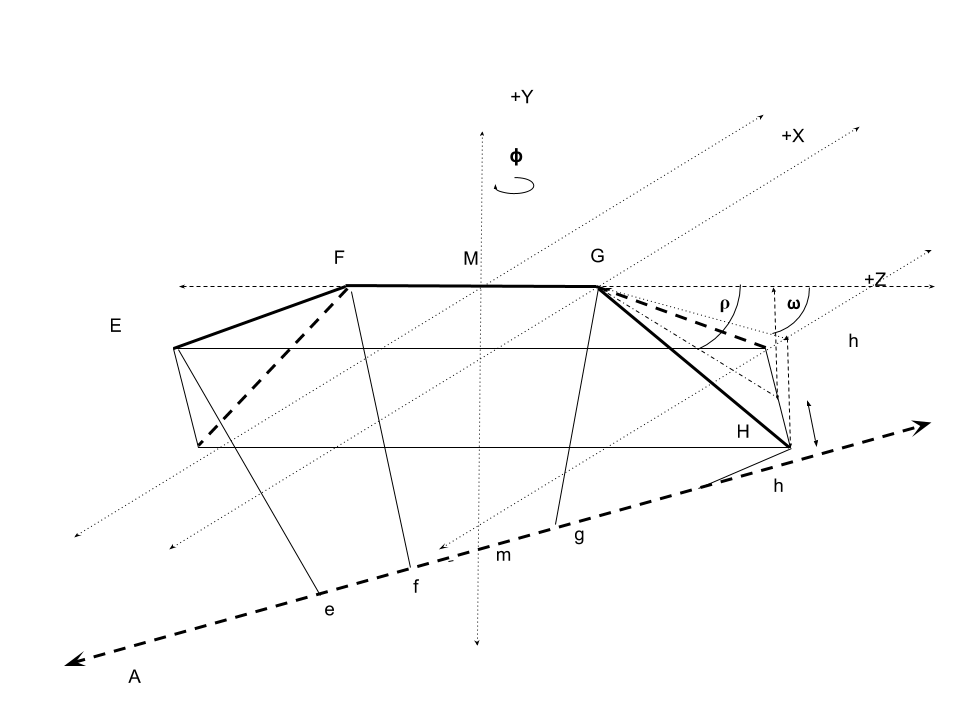
\includegraphics[width=0.80\textwidth]{figures/TwoAngleDiagram.png}
     \caption{Three Symmetric Members}
  \label{fig:threemembersdiagram}
\end{figure}

Kahn\cite{kahn1989defining} has given a method for computing the axis of a helix in the context of chemistry.
This method uses the observation that the angle bisectors of the segments on a segmented helix are perpendicular
and intersect the axis of the helix.
Because the helices may not be perfect and because the measurement of positions may not be perfectly accurate,
it is common for chemists to use regression and fitting methods to fit helix parameters to observed positions
on the helix.
Kahn's method was a prelude to some error-tolerant methods applicable to
the realm of organic chemistry.
In this paper we are concerned with pure geometry. Also, Kahn was writing in 1989,
and we now have more convenient computing tools. We give here a modification of Kahn's algorithm, called {\em PointAxis},
which relies on our ability, working in the realm of pure geometry, to position the segments on the axes
to simplify the derivation and computation.

\subsection{A Sketch of the 4-Point Method}

Using tools from linear algebra and well-documented algorithms, a sketch of the finding the segemented helix from
four consecutive known points $A,B,C,D$ is:
\begin{itemize}
\item Compute the bisectors of the angle $B_b$ of $ \angle{ABC}$ and the angle $C_b$ of $\angle{BCD}$.
  If the points are collinear, we have a special case.
\item Because these angle bisectors point at the axis of the segmented helix, their cross product is a vector
  in the direction of the axis. If $B_b$ and $C_b$ are parallel or anti-parallel the cross product is not defined
  and we have special cases.
\item  Otherwise the vectors $B_b$ and $C_b$ are skew, the algorithm for the closest points on two skew lines provides two points $B_a$ and $C_a$ on these vectors which
  are the closest points on on those lines and are also points on the axis.
\item The distance between $B_a$ and $B$ is the radius, and the distance between $B_a$ and $C_a$ is the travel $d$ along the axis.
  \item The angle between $B - B_a$ and $C - C_a$ is $\theta$.
  \end{itemize}

\subsection{The 4-Point Test}

It is useful to have a test if four proposed points really do lie on a segmented helix.

\begin{theorem}[Segmented Helix Test]
  Four arbitrary sequential points $A,B,C,D$ are consecutive joints of a segmented helix if and only if
  they segments $\overline{AB},\overline{BC}$, and $\overline{CD}$ are equal length and the scalar projection
  of $\overline{CD}$ onto $\overline{BC}$ is equal to the negation of the scalar projection of $\overline{AB}$ onto $\overline{BC}$.
\end{theorem}

\begin{proof}
  Case ($A,B,C,D$ on segemented helix implies negation of scalar projections):

  By Chasles' Theorem, there is a screw $S$ that takes $\overline{AB}$ into $\overline{BC}$, and a screw $R$ that
  takes  $\overline{CD}$ into $\overline{BC}$. If $R$ is the negation of $S$, the projections will be the same.

  If the projections are the same, there is a midpoint. Without loss of generality, rotate around $\overline{BC}$ so that
  the midpoint points straight down. Now $A.x = -D.x$, if the projections have the same length. If this is is so, the
  screw that takes $\overline{CD}$ into $\overline{BC}$ ($R$) has the same magnitude of rotation as $S$.
  The direction vector of $S$ points in the opposite direction to $R$. The distance travelled is the same, therefore $R$
  is the negation of $S$.

  Case (equality of scalar projection implies a segmented helix):

  To Be Done

\end{proof}

\subsection{The 4-Point Method}

Therefore four consecutive points completely determine at least one segmented helix. We will concern ourselves
only with the helix that makes the least rotation between points.
We provide a modification of the PointAxis algorithm
with takes four such points (without loss of generality $B$ and $c$ are assumed to be centered on the $z$-axis, and that a
rotation has been performed to balance $A$ and $D$ to that $A.x = -D.x, A.z = - D.z$, and $A.y = D.y$. Thus the input to
PointsAxis in fact has three only three degrees of freedom, which determine the three intrinsic propoerties $r,d,\theta$
which completely define the shape of a segments helix (but not its location in space.)


In the derivations below, we rely on certain facts about
the segmented helix formed by the stack of objects, the first
of which is key:
\begin{itemize}
\item Without loss of generality, we may think of any member whose faces
  and twist generate a non-degenerate helix as being ``above'' the
  axis of the helix. We furthermore choose to place the object in
  this figure so that $B_y = C_y$, that is, that the members are symmetric
  about the $z$-axis.
  $A$ and $D$ are ``balanced'' across the $YZ$-plane,
  and $A_x = -D_x$ and $A_y = D_y$.
\item Every joint ($A,B,C,D$) is the same distance $r$ from the axis $H$ of the helix.
\item Every member is in the same angular relation $\phi$ to the axis of the helix.
\item Since every member cuts across a cylinder around the axis,
  the midpoint of every member is the same distance from the axis
  which is general a little a less than $r$. In particular the midpoint $M$
  whose closest point on the helix axis $m$ is on the $y$-axis and
  $\overline{Mm} < \overline{Bb}$.
\item The points ($A_a,B_a,C_a,D_a$) on the axis closest to the joints ($A,B,C,D$)
  are equidistant about the axis and centered about the $y$-axis. In
  particular, $\| \overline{B - B_a} \| = \| \overline{C - C_a} \|$.
\end{itemize}

From the observations that $\| \overline{B - B_a} \| = \| \overline{C - C_a} \|$
we concluded that the helix axis is in a plane
parallel to the $XZ$-plane, it intersects the $y$-axis, but in general is
not parallel to the $z$-axis.

Because the angle bisectors of each joint are in general skew, and intersect the
axis perpendicularly, it is clear we can use linear algebra and the algorithm
for the closest points on two skew lines to find $B_a$ and $B_c$.

However, we can take advantage of the fact that a segmented helix has
tremendous symmetry, and the angle bisectors are very far from being two
generally skew lines. In fact, by taking advantage of the fact that the
generating rule for an object chain requires similarity in every joint,
we can arrange the objects as in Figure \ref{fig:threemembersdiagram}.

PointAxis takes a length and a point $D$ known to be in
a specific relation to $B$ and $C$.

We have carefully arranging our axes
so that we can compute $\phi$, the angle between the helical axis
and the $z$ axis. This, in combination with symmetry and the knowledge
that the helical axis is in the $XZ$ plane, lets us compute the
points on the axis corresponding to the joints directly from $\phi$.

This algorithm coded below, is simple enough that Mathematica can
actually produce symbolic closed-form formula for all computed valued
in terms of $L, x, y, z$, but they are less comprehensible to the
human eye than this algorithm, although their existence opens
the possibility that, for example, the derivative representing
the change in $r$ with a change in $D$ could be calculated.

\subsection{Degenerate Cases}

The fundamental insight that the axis of the helix $H$ can be
computed by a cross product of the angle bisector
vectors ($Bb$ and $Cb$) applies only
when the angle-bisectors have a non-zero length and when
they are not anti-parallel. When the are of zero length, this is
the degnerate case of a straight line coinciding with all segments.
This occurs only when $z = L$.
When $Bb$ and $Cb$ are parallel (pointing in opposite directions),
the zig-zag degeneracy occurs. This occurs only when $y = 0$.

Once $H$ has been calculated, the signed travel along the axis $da$ is
the scalar projection of a segment $(C - B)$ onto $H$.
From this $\phi$ is directly calculatable. $\phi$ allows
a direct calculation of the $x,y$ and $z$ components of the
point $Ba$ on the axis pointed to by $Bb$.
$r$ is the distance between $Ba$ and $B$. $c$ and $\theta$
are easily computed from these values.

TODO: Move the tests that I have coded in JavaScript into
Mathematica, handle special cases as separate math routines
to report here.

\begin{lstlisting}
ChordFromLDaxis[L_,Da_] := Sqrt[L^2 - Da^2]
RotationFromRadiusChord[R_,C_] := 2 ArcSin[C/(2R)]
PointAxis[L_,{x_,y_,z_}] := Block[{A, B, C, D, Cb, Bb, H,
                                  Bax, Bay, Baz, Ba,
                                  r, theta, da, c, phi},
  D = {x,y,z};
  A = {-x, y, -z};
  B = {0, 0, -L/2};
  C = {0, 0, L/2};
  Cb = (B+D)/2 - C;
  Bb = (A+C)/2 - B;
  H = Normalize[Cross[Bb,Cb]]; // Why am I calling Normalize twice?
  da = (C - B) . Normalize[H];
  phi = ArcCos[da/L];
  Bax = Sin[phi] da / 2;
  Baz = -Cos[phi] da / 2;
  Bay = Bb[[2]] (Bax / Bb[[1]]);
  Ba = {Bax,Bay,Baz};
  r = Norm[Ba - B];
  c = ChordFromLDaxis[L,da];
  theta = RotationFromRadiusChord[r,c];
  {r,theta,da,c,phi,H}
]
\end{lstlisting}

Note that in Figure \ref{fig:threemembersdiagram} there is great
room for confusion in terms of plane $\omega$ is actually
measured against. The three triangles $\triangle BB_aC$, $\triangle BM_aC$, and $\triangle BM_aC$
are all in general not co-planar, that is, they are all at
slight angles to each other.

There is one reason one might prefer the transformation matrix method or the point method over the other: with modern
computer algebra systems such as Mathematica it might be possible to use these ``algorithms'' to produce closed-form
expressions of closed-form (alebraic) inputs. For example, the Platonic solids all have lengths and face normals which
can be specificed exactly in closed (thought irrational) form. Thus it might be possible to produce an expression for the
radius of one of the Platonic Dodecahelices of unit edge length. We have not understaken this work.


\section{The Face Normal Method}
\label{sec:facenormal}

PointAxis takes a point $A$ known to be in a specific, balanced relation
to $B$ and $C$. A chemist might know 4 such points from crystallography,
and be able to move them into this symmetric position along the $z$-axis.

However, we might instead know something of the subunits and
how they are conjoined, without actually knowing where points $A$
and $D$ are.


\begin{figure}
     \centering
     \includegraphics[width=0.80\textwidth]{figures/ObjectForStackingSetup.png}
     \caption{The rotatable prism of three objects}
  \label{fig:intrinsicdiagram}
\end{figure}

\begin{figure}
     \centering
     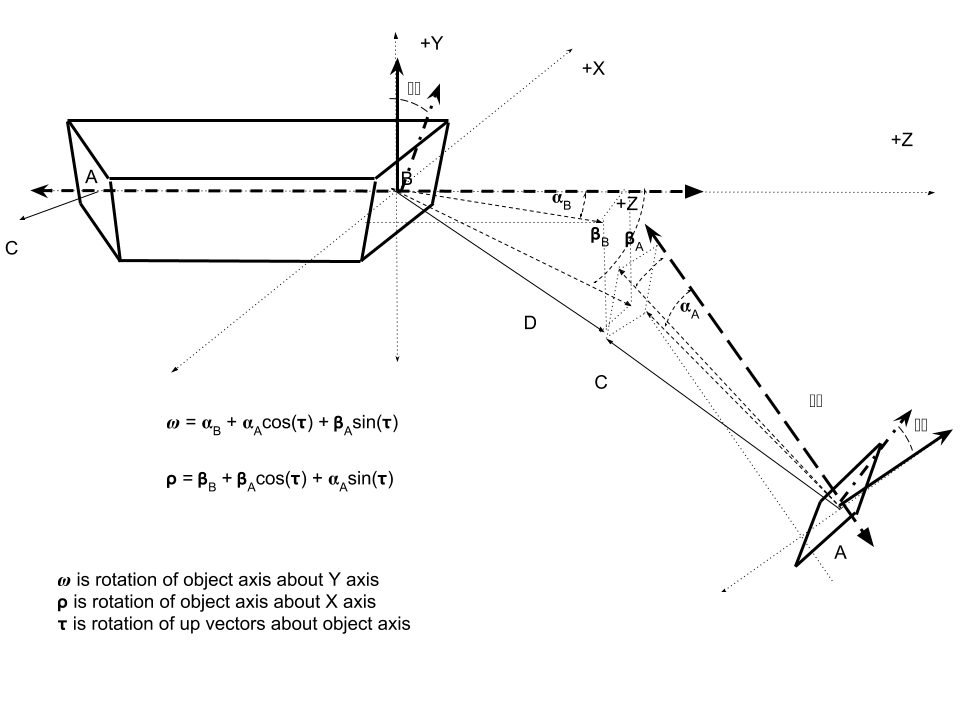
\includegraphics[width=0.80\textwidth]{figures/JointGeometry.png}
     \caption{Joint Geometry}
  \label{fig:jointdiagram}
\end{figure}


We start with these intrinsic properties of an object, and additionally the
rule for how objects are laid face-to-face. That is, knowing the length between two
joint points and a vector normal to the faces of the two joints, we almost have
enough to determine the unique stacking of objects. The final piece is that we must
know the {\em twist}. That is, when face $A$ of a second objects is placed on face $B$
of a first object so that they are flush (that is, their normals are in opposite directions),
it remains the case that the second object can be rotated about the normals. To
define the joining rule, we must attach an {\em up vector} to each object. Then a joining
rule is ``place the second object against the first, joint point coincident to joint point,
and twist it so that its up vector differs by $\tau$ degrees from the up vector of the first
object.'' In this definition, the up vectors are considered to be measured against the plane
containing the two axes meeting in a joint.

Define the {\em joint plane} to be the plane which contians the two axes meeting in a joint.
Define the {\em joint line} to be the line throught the joint perpendicular to the joint plane.
Define the {\em joint angle} to be the angle of the first axis to the second measured about
the joint line.
The twist $\tau$ is the change in the a vector attached to the object rotated about the joint
line by the joint angle. That is, take any vector attached to the first object, place it at
the joint, rotate it about the joint line via the joint angle. $\tau$ is the difference
between the angle of this vector measured against the joint plane and the angle of the
up vector of the second object measured against the joint plane.

If the objects are macroscopic objects which have faces, this is the same as the rotation
of the axis of the second object relative to the first in the plane of the coincident faces.
We can indentify intrinsic properties:

\begin{itemize}
\item An object with two identified faces, labeled $B$ and $C$. Assume there normalized
  vectors $N_B$ and $N_C$
  from each of these points that is aligned with the axis of the conjoined object attached to
  that face. This normals might be enforced by the fact that flat faces are joined in the joint plane.
  However, molecules don't have faces; this conjoining relationship may be enforced some other way.
\item The length $L$ of an object, measured from joint point $A$ to joint point $B$.
\item A joint twist $\tau$ defining the change in computed out-vector between objects,
  measured at the joint face.
\end{itemize}

\subsection{Rotating into balance from face normal vectors}

In order to use the PointAxis algorithm, we need a way
to compute points $A$ and $D$ in balance around the axis $BC$.
A key insight is that Lord's Observation tells us that no matter how lopsided and different
the normal vectors  $N_B$ and $N_C$ for the joint faces are and no matter what $\tau$ we choose,
when we conjoin objects
their relationship is always the same.
After placing $BC$ along
the $z$-axis, there is always an angle $\psi$ which will
rotate the points $A$ and $D$ into balance (that is, $(A.x = -D.x) \wedge (A.z = -D.z) \wedge (A.y = D.y)$.

For computer programmers with a graphics library supporting transformation matrices such
as THREE.js\cite{dirksen2013learning},
it is relatively easy to code the math to adjoin objects
face-to-face based on the face normals, simulating the physical act of
matching flat faces between macroscopic objects.
\begin{enumerate}
  \item Create the transformation the aligns and centers $\overline{BC}$ on the $z$-axis.
\item Create a translation of $B$ to $C$.
\item Create a rotation of the $z$-axis to  $N_B$.
\item Create a rotation of of $-N_c$ about $N_B$.
  \item Create a rotation of $\tau$ around that axis.
\end{enumerate}
Composing these transformation matrices via multiplication creates a
transformation matrix which takes $B$ to $C$ and $C$ to $D$.

We will assume this
as a subroutine called ``adjoinPrism'' which takes $\tau$
(the rotation inside the plane of the joint). A byproduct
of balancing the points is the a transformation matrix
that takes $C$ into $D$. Having done this, one can compute
the screw axis, and hence all of the segmented helix properties,
from either the transformation matrix or the four points. Our
code does both and compares the result as a test.

The key insight to finding $\psi$ to note that we
can consider the projections of the $B$ and $C$ face normal vectors
projected into the $XY$ plane, and rotate these so that they
are balanced around the negative $y$ unit vector. Even
if the lengths of the projections of the face normals in $XY$
are different, this mechanism works.

By composing this balancing operation with the face-adjoining transformation
matrix, $A$ and $D$ are placed in balance. The screw axis may now
be computed from either the four points $A,B,C,D$ or from the transformation
matrix created to balance them.

\subsection{On the Choice of the Screw Axis Direction}

Given only a physical segmented helix without position in space, we may arbitrarily choose the
direction for the axis. Changing our decision will make the screw axis point in the negative direction,
change the sign of the travel $d$ along the axis, and choose $\phi$ to be $\pi - \phi$.

As can be seen from interactive play with our software, it is entirely possible for the travel along
the axis of the helix to be $0$--in fact, choosing $\tau \approx 0$ produces toruses, which have no
travel along the axis.

We could represent this be makng the length of the vector representing the axis be the length of the
travel $d$. However, this would have the drawback than when $d$ is zero we would be unable to determine
the axis of revolution of the torus. Although somewhat arbitrary, I have chosen instead to represent the
axis as a normalized vector of unit length, and to allow the travel to be negative. This has the value that
chaning $\tau$ through zero smoothly changes $d$. However, it creates the problem that as $\tau$ approaches
$\pi$ from different directions the signs of the axes are different. That is, $\tau = \pi$ and $\tau = -pi$ decscribe exactly
the same shape, but in our calculation they will have different signs for the axes. The radius, pitch and
absolute value of the travel,
which are intrinsic to the shape, will be the same, but the axis vector, $\phi$, and the sign of $d$ will be different.

\section{Checks and Explorations}

Note: It is useful to compute $\psi$, the direction angle of
the midpoint of the projections of the face normals.
We also need to define the differences between these angles
as well $\delta$.
Choosing $\tau$ so that the $\delta$ is zero produces a torus-like
structure. Choosing $\tau$ so that $\delta$ is 180$\degree$ produces
the zig-zag case, which is of maximum travel.


\subsection{Changing $\tau$ Smoothly Changes Tightness}

\begin{theorem}[Twist Spectrum]
  For any choice of face normals having non-zero $x$ or $y$ components, changing $\tau$ smoothly varies the segmented helix
  between a torus and zig-zag cases.
  \end{theorem}

\begin{proof}
  By interactively manipulating the software it is apparent.
  \end{proof}

\begin{theorem}[Torus Corollary]
  For any choice of face normals, there is choice of the twist $\tau$ for which the segmented helix is a planar polygon,
  thereby resembling a torus.
  \end{theorem}

\begin{proof}
  By interactively manipulating the software it is apparent.
  \end{proof}

TODO: Can we calculate the $\tau$ value as a function of the face normals? That would make a nice little constructive theorem.


In this section add graphs. Also, a check against the BC helix.
Possibly software should be used to produce a 3D simulation
of the issues.

Idea: Define ``tightness'' to be $ p / r$, where $p$ is pitch and $r$ is radius. Attempt to prove that in some ways tightness increases with increasing $\tau$.

\subsection{Qualitative observations}

Varying $\tau$ smoothly varies the tightness of the coiling of the helix, moving through vary linear cases towards a torus,
to a torus, to a very linear case on the other side.

In fact it is possible to that there is always a ``tightest coil'' which does not self-intersect. If we had many objects,
we could pack them into a conveneient space by computing the $\tau$ of the tightest coil and stacking them this way.
If we had a means to change $\tau$, perhaps via motors in a robot arm, we would have a smoothly telescoping and contracting
robot arm.


\section{Applying to The Boerdijk-Coxeter Tetrahelix}

The Boerdijk-Coxeter tetrahelix is a periodic chain of conjoined regular tetrahedra
which has been much studied\cite{coxeter1985simplicial,sadler2013periodic,fuller1982synergetics,read2018transforming} and happens to have irrational measures, making it an ideal
test case for our algorithms. Because the face-normals can be calculated and the
positions of the elements of the BC helix directly calculated, we can use
it to test our algorithms, and in fact these algorithms give the correct result.

However, it should be cautioned that the helix which Coxeter identified\cite{coxeter1985simplicial} goes through every node of every tetrahedron. Constructing the helix that goes
through only ``rail'' nodes allows the tetrahelix to be modified\cite{read2018transforming}.
However, the segmented helices defined in this paper do neither; rather, it is most natural to
imagine them moving through the centroid of face of a tetrahedron.
This complementary view is to think of the BC Helix not as the helix that
intersects the vertices of the tetrahedron as Coxeter did\cite{coxeter1985simplicial}, nor a single
rail as may be valuable to engineers\cite{read2018transforming}, but rather as a helix through
the center point of the faces of the tetrahedron. This is a segmented helix of
very small radius compared to the other two approaches, but it has
the advantage that it is far more general. For example, it is
clearly defined if one used truncated tetrahedra.
The rotation of a
segment thus matches the BC Helix ($\arctan{-3/2}$), but the radius of the
generating segmented helix in the paper would be smaller than those segmented helices that intersect the nodes.

In light of Lord's observation and the Segmented Helix algorithms, we can now
consider the BC Helix, and in fact a variety of segmented helices generated by
face-to-face stacking of Platonic solids, examples of called {\em Platonic segmented helixes}.

Note this also makes clear that in these cases we must also specify the {\em twist},
even if we insist on perfect face-to-face matching. Thinking of it this
way, there are actually three tetrahedral segmented helices, depending on which twist 120$\degree$
is chosen (keeping the faces matching). In the case of the tetrahedron,
this creates the clockwise BC Helix, the anti-clockwise BC Helix, and the
not-quite-closed tetrahedral torus.

In the case of the icosahedron, there are in fact many possibilities,
as one need not choose the precisely opposite face as the joining face, and
one may choose up to three twists. The ``zoo'' or Platonic helices
can be studied via the calculations described here, and our software
makes these interactively selectable (see Section\ref{sec:platonic}).

\section{Implications}

One of the implications of having an easily-calculatable understanding of the math
is that it may be possible to design helixes
of any radius and pitch by designing periodic (possibly scalene) segments. Combined with slight
irregularities, this means that you have a basis of design molecular helices
out of ``atoms'' which correspond to our objects.

This would mean that if you wanted to build a brace of length exactly 3 meters
with bars of exactly 1/2 meter you would be able to come as close to this
as mathematically possible.

A modular robot constructed out of repetitions of the same shape-changing module will always product a helix
whose precise shape can be controlled by uniformly changing the shape of all of the modules.

\section{The Platonic Helices}

\label{sec:platonic}

In order to demonstrate the utility of the calculations explained in this paper, we have explored
periodic chains of the five regular Platonic solids joined face-to-face so that their vertices coincide,
which form {\em Platonic helices.}
Such tetrahelices, icosahelices, octahelices and dodechelices
have been mentioned in a number of papers\cite{elgersma2016quadrahelix,babiker2012combinatorial,lord2001sphere}, but not exhaustively studied in
the purely helical form.
We propose the name {\em cubahelix} for the helix made from cubes, as opposed to the equivalent
but cumbersome {\em hexahedronahelix}.
Because in some cases Platonic segmented helices may be found in nature or
related to structures found in nature\cite{lord2004gamma,pearce1990structure},
it would be convenient to have a table, and images, of all such Platonic segmented helices for reference.

To construct a periodic chain from a Platonic solid, one must decide which faces are joined by the rule.
Additionally, one must determine a twist
$\tau$ as part of the rule, and this twist must be chosen from a small set if the vertices are to coincide.
The set of vertex-matching twists differs slightly depending on the face chosen for octahedron, dodacahedron, and icosahedron
(but not for the tetrahedron and the cube.) The of twists set will always be equal to the number of sides on a face.

Therefore the number of Platonic helices is in principle a summation of a number of faces times a number of sides, or
$4 \cdot 3 + 6 \cdot 4 + 8 \cdot 3 + 12 \cdot 5 + 20 \cdot 3 = 12 + 24 + 24 + 60 + 60 = 180$.
However, many of the possibly helices will be indistinguishable of we consider only the shapes produced. Furthermore,
every non-toroidal helix will come in clockwise and counter-clockwise version.
However, we do not consider rules such as ``attach face zero to face zero''.
The transformation matrix for such a rule would be the identity matrix.
It produces an object axis of zero length, a radius of zero, and
a travel of zero. It produces perfect self-intersection; that is the entire
degenerate helix would appear to be a simply a single Platonic solid.

Using the math in this paper, it was easy to evaluate all 180 helices,
place them in table, and group them
by radius and travel (collapsing chirality).
The result is 27 unique shapes. In this number, no provision was made to exclude
self-intersection,
which does occur, but might not matter to
an aerospace engineer building a collapsible space frame of rods and joints.


With those caveats, the resulting table and accompanying figures thus represents an exhaustive catalog,
commonly called a ``zoo'' today, of all Platonic
helices in Table \ref{table:platonic}.
Many of the these helices have been previously mentioned and even rendered in the literature,
but as far as we know have not been cataloged. In this table, column {\em C-Face} refers to the
face as numbered by the THREE.js software\cite{dirksen2013learning}, which is somewhat arbitrary. The {\em \# Analogs}
column gives the number of Platonic Helices with the same shape, or the enantiomer of it, that is, the same
shape in either the clockwise or anticlockwise direction. This list can be expanded completely in our interactive software.

Clearly, for each solid there is a change in twist which keeps the faces aligned if they start aligned. This is the $2\pi/n$,
where $n$ is the number of sides in a face. It is perhaps surprising, though, that the base twist that creates
a perfect face-to-face match depends not only on the solid but the face we choose to conjoin to. For each of the Platonic
solids, we have just computed thihs base angle by visual inspection and trial and error. The twist $\tau$ if a species
of helix in given in the column below.

\begin{table}[ht]
\caption{The Platonic Helices} % title of Table
\centering % used for centering table
\begin{tabular}{l l r r r r r r r}
  \hline\hline %inserts double horizontal lines
  Name & Solid & \# Analogs & C-Face \# & $ \tau $ & radius & d & $ \phi $ & $ \theta $	\\ [0.5ex] % inserts table
%heading
  \hline % inserts single horizontal line
Tetrahelix & Tet &	6 &	1 &	-120 &	0.094 &	131.810	& -0.516 & 161.565 \\
Tetratorus & Tet & 	3 &	1 &	0    &	0.471 &	70.529	& 0.000	& 90.000 \\
\hline %inserts single line
Boxbeam & Cub &	4 &	1 &	-180 &	0.000 &	0.000 &	1.000 &	0.000 \\
Staircase & Cub &	4 & 	2 &	-180 &	0.000 &	0.000 &	0.707 &	0.000 \\
Blockhelix & Cub & 	8 & 	2 & 	-90  &	0.236 &	120.000 & -0.577 & 144.736 \\
Cubatorus & Cub &	4 &	2 &	0 &	0.500 &	90.000 & 0.000 & 90.000 \\
\hline %inserts single line
Octabeam & Oct &	3 &	5 &	-60 &	0.000 &	0.000 &	1.155 &	0.000 \\
Octaspikey & Oct &	6 &	1 &	-120 &	0.148 &	146.443 & -0.603 & 154.761 \\
Octamedium & Oct &	6 &	2 &	-120 &	0.163 &	131.810 & -0.894 & 161.565 \\
Octagear & Oct &	3 &	1 &	0 &	0.408 &	109.471 & 0.000	& 90.000 \\
Treestar & Oct &	3 &	2 &	0 &	0.816 &	70.529 & 0.000 & 90.000 \\
\hline %inserts single line
Dodecabeam & Dod &	5 &	8 &	-108 &	0.000 &	0.000 &	1.589 &	0.000 \\
Dodecadoubler & Dod &	10 &	1 &	-144 &	0.113 &	161.301 &-0.805 & 164.550 \\
The Alternater & Dod &	10 &	2 &	-144 &	0.118 &	149.520 &-1.333	& 170.306 \\
Dodecashaft & Dod &	10 &	1 &	-72 &	0.351 &	129.657	&-0.543 & 130.501 \\
Dodecagear & Dod &	5 &	1 &	0 &	0.491 &	116.565	& 0.000	& 90.000 \\
Dodecacorkscrew & Dod &	10 &	2 &	-72 &	0.546 &	93.026 & -1.095 & 144.110 \\
Dodecadonut & Dod &	5 &	2 &	0 &	1.286 &	63.435 & 0.000 & 90.000 \\
\hline %inserts single line
Pearlshaft & Ico &	3 &	13 &	-60 &	0.000 &	0.000 &	1.589 & 0.000 \\
Quasi-planar & Ico &	6 &	8 &	165 &	0.049 &	167.764 & 1.294 & 4.347 \\
Two Strands & Ico &	6 &	1 &	120 &	0.137 &	159.446	& 0.499 & 28.340 \\
Slow Twist & Ico &	6 &	12 &	120 &	0.169 &	124.309	& 1.454	& 11.641 \\
Rock Candy & Ico &	12 &	2 &	120 &	0.204 &	146.443	& 0.830 & 25.239 \\
Icosa Tree Star & Ico &	3 &	1 &	0 &	0.304 &	138.190	& 0.000	& 90.000 \\
Icosacorkscrew & Ico &	6 &	8 &	-75 &	0.512 &	99.253	& -1.037 & 143.042 \\
Planar point cluster & Ico &	6 &	2 &	0 &	0.562 &	109.471 & 0.000 & 90.000 \\
Big Icosacorkscrew  & Ico &	6 &	8 &	45 &	0.803 &	82.064 & 0.756 & 54.343 \\
The Wheel & Ico &	3 &	12 &	0 &	2.080 &	41.810 & 0.000 & 90.000 \\
\hline %inserts single line
\end{tabular}
\label{table:platonic} % is used to refer this table in the text
\end{table}

\subsection{Qualitative Descriptions and Interesting Shapes}

For fun and to facilitate conversation, we have given all 27 of these Platohelices nicknames that we find descriptive.
A few of these are interesting enough
to be worthy of particular mention, and comparing them shows the possibility of designing structures using nothing but Platonic solids.
The math in this paper works equally well with irregular shaps as well, allowing continuous spectra of designed structures from repeated shapes
or molecules.

\begin{itemize}
\item ``The Blockhelix'' (Figure \ref{fig:blockhelix}) is cubic rectilinear structure in which all angles are right angles; nonetheless
  a segmented helix hides inside it perhaps not apparent to the human eye at first glance.
\begin{figure}
     \centering
     \includegraphics[width=0.40\textwidth]{figures/Blockhelix.png}
     \caption{The Blockhelix}
  \label{fig:blockhelix}
\end{figure}

\item ``Pearlshaft'' (Figure \ref{fig:pearlshaft}). Conjoining parallel faces always produces a {\em shaft}. This icosahedron, being relatively round,
  resembles a string of pearls.
\begin{figure}
     \centering
     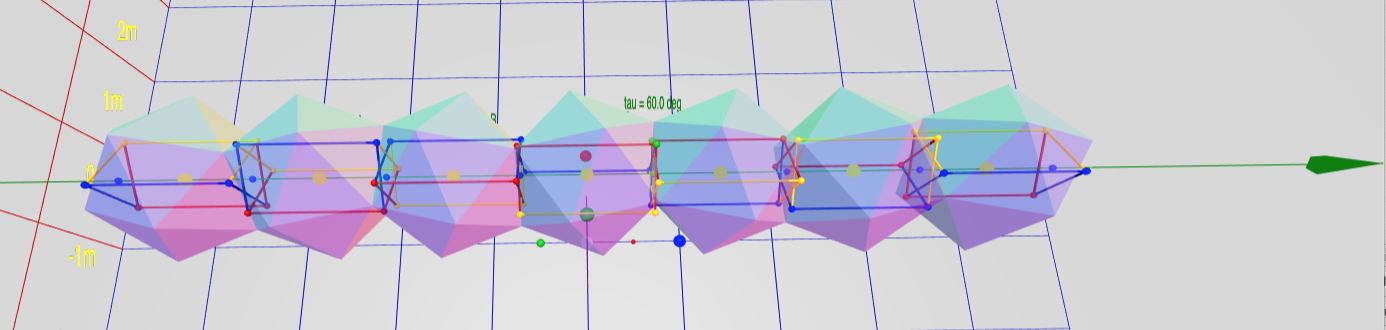
\includegraphics[width=0.40\textwidth]{figures/PearlShaft.png}
     \caption{The Pearlshaft}
  \label{fig:pearlshaft}
\end{figure}

\item However, shaft-like helices exist which do not join opposite faces. ``The Dodecashaft'' (Figure \ref{fig:dodecashaft}) is a remarkably tight
  non-self-intersecting dodecahelix with very narrow gaps between objects.
  Such a configuration
  might be formed by nanofibers under pressure.
\begin{figure}
     \centering
     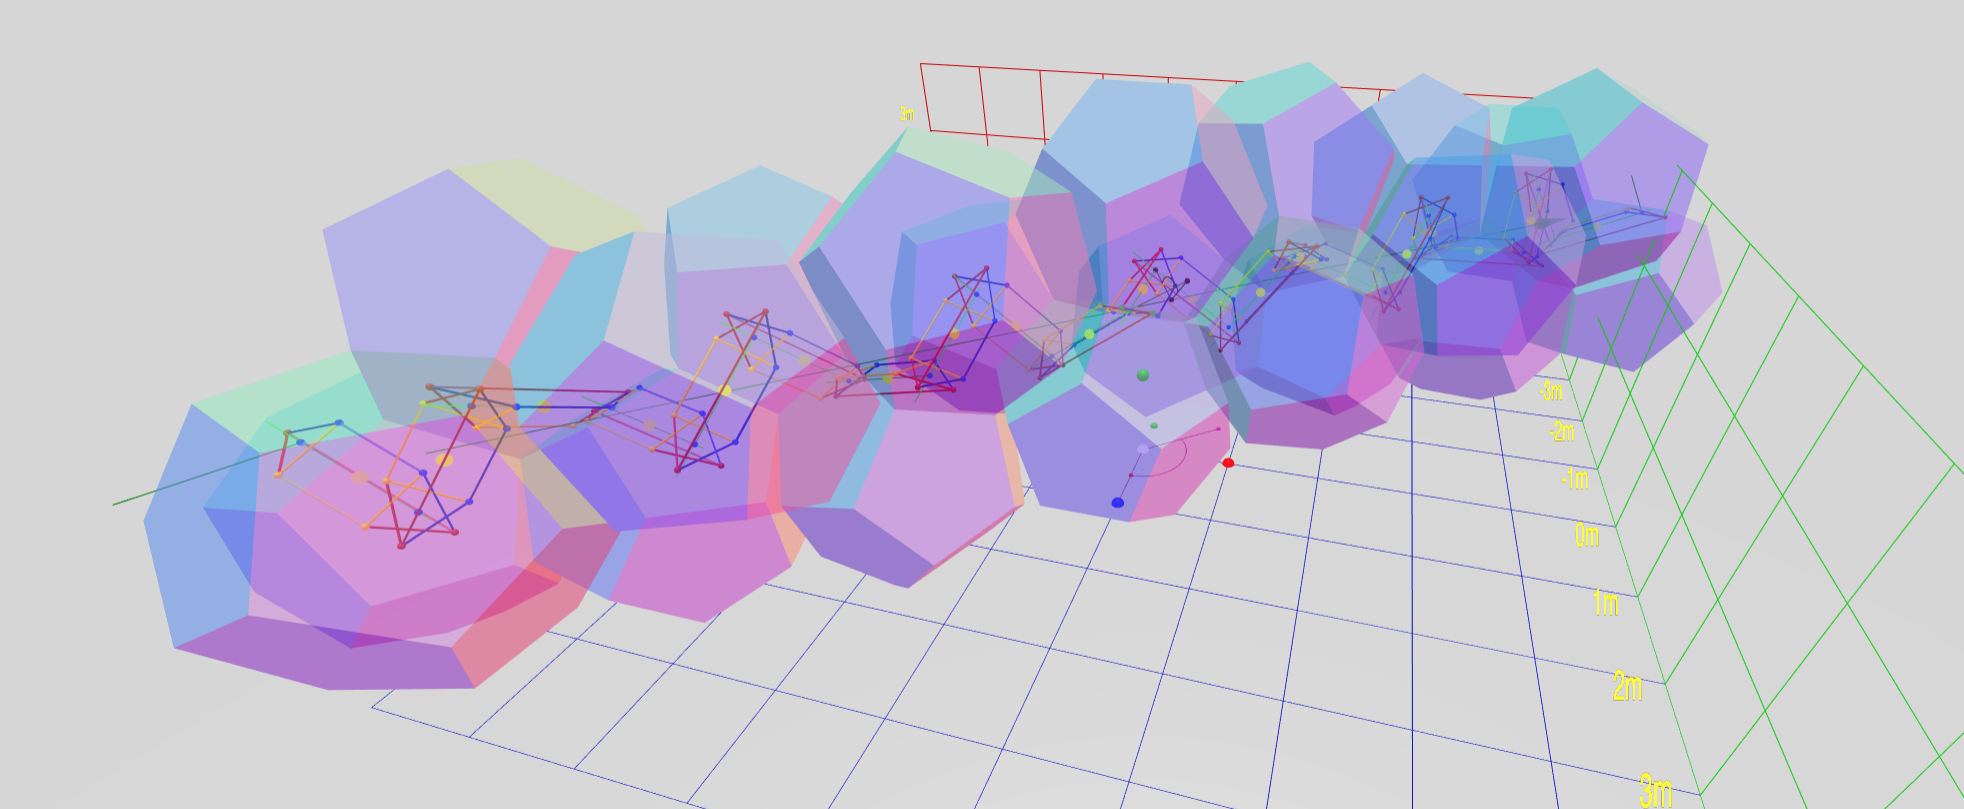
\includegraphics[width=0.40\textwidth]{figures/Dodecashaft.png}
     \caption{The Dodecashaft}
  \label{fig:dodecashaft}
\end{figure}
\item ``The Dodecadoubler'' (Figure \ref{fig:dodecadoubler}) presents the appearance of being a double helix, even though in fact it is a single helix with
  a simple twist of 72 $\degree$ from the Dodecashaft
\begin{figure}
     \centering
     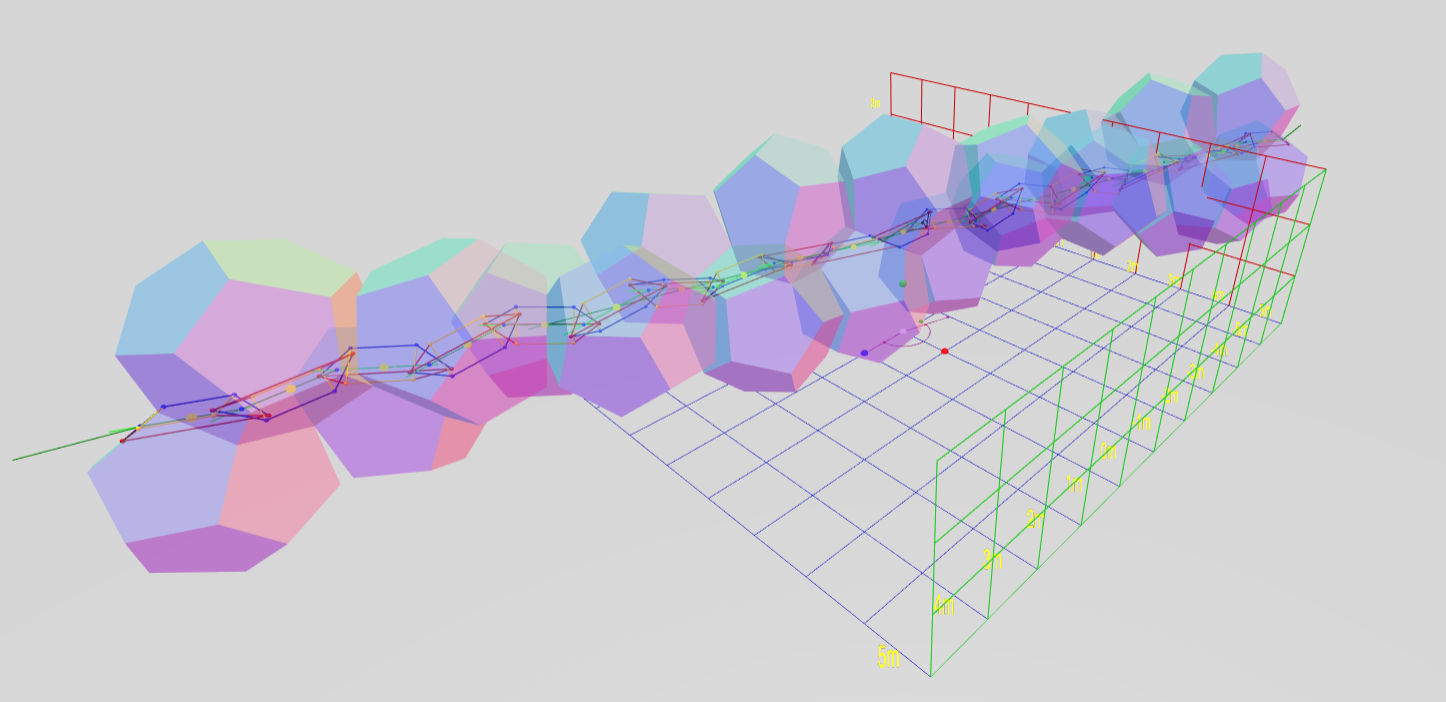
\includegraphics[width=0.40\textwidth]{figures/Dodecadoubler.png}
     \caption{The Dodecadoubler}
  \label{fig:dodecadoubler}
\end{figure}
\item ``The Dodecacorkscrew'' (Figure \ref{fig:dodecacorkscrew}) is a contrasting example of a loose helix, reminiscent of a corkscrew for opening wine bottles.
\begin{figure}
     \centering
     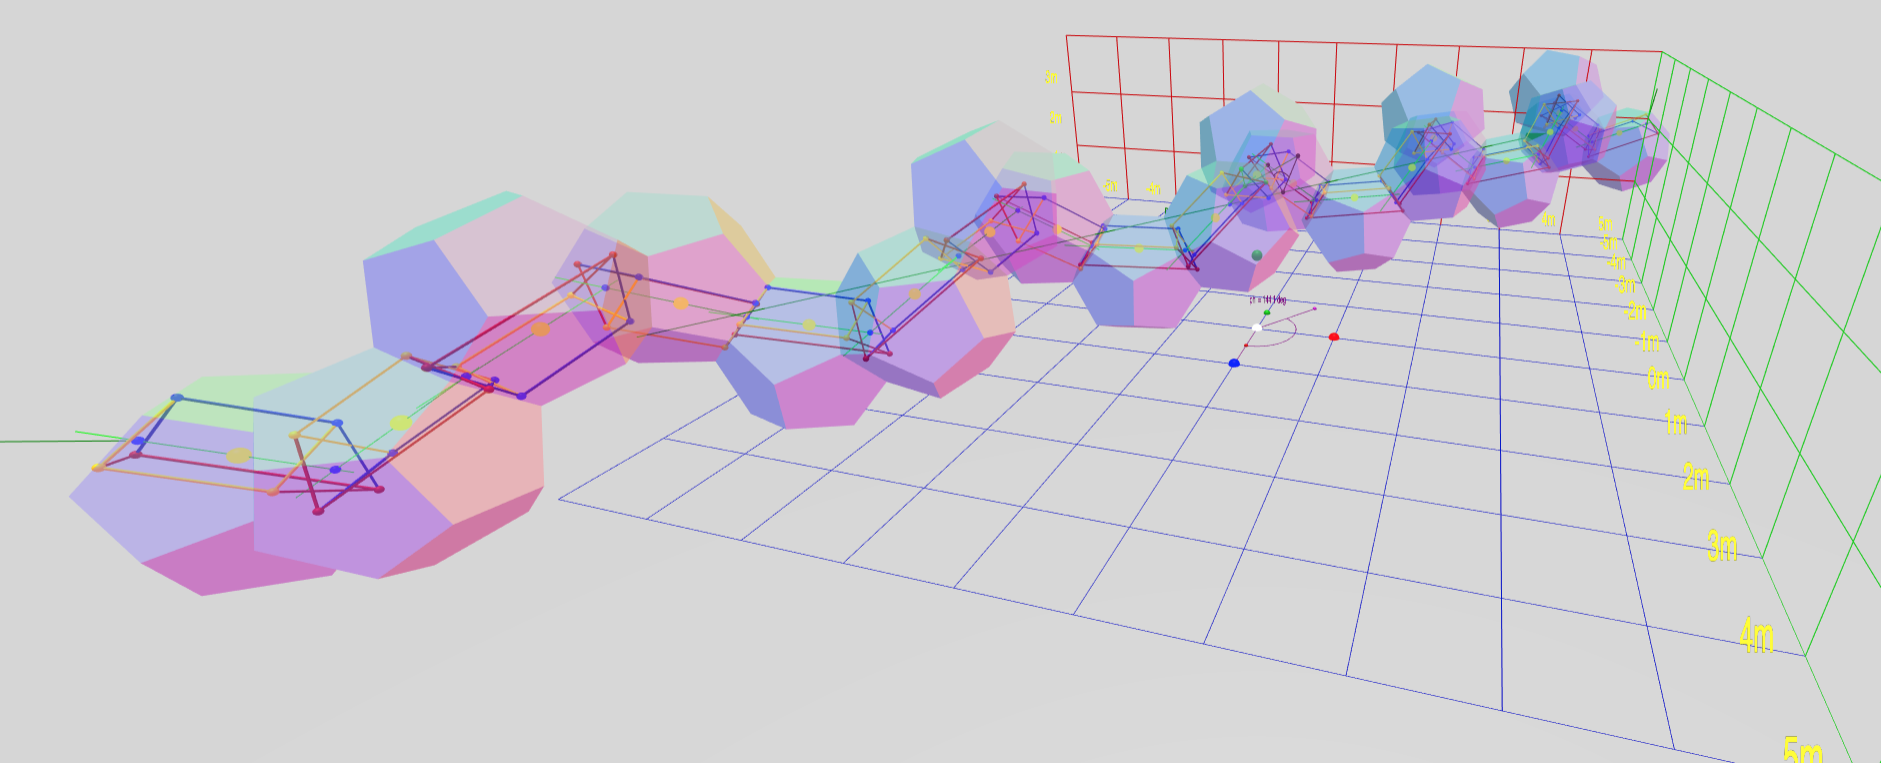
\includegraphics[width=0.40\textwidth]{figures/Dodecacorkscrew.png}
     \caption{The Dodecacorkscrew}
  \label{fig:dodecacorkscrew}
\end{figure}
\item The ``Quasi-planar'' (Figure \ref{fig:quasiplanar}) icoshelix presents a slowly twisting metahelix, so perhaps 10 icosahedron could be said to ``lay flat''. If this were
  a molecule or a physical structure made of less-than-perfect rigid members it migt be possible to force it into a pure planar configuration,
  thus wrapping a cylinder or a plane, studding it with icosahedra.
\begin{figure}
     \centering
     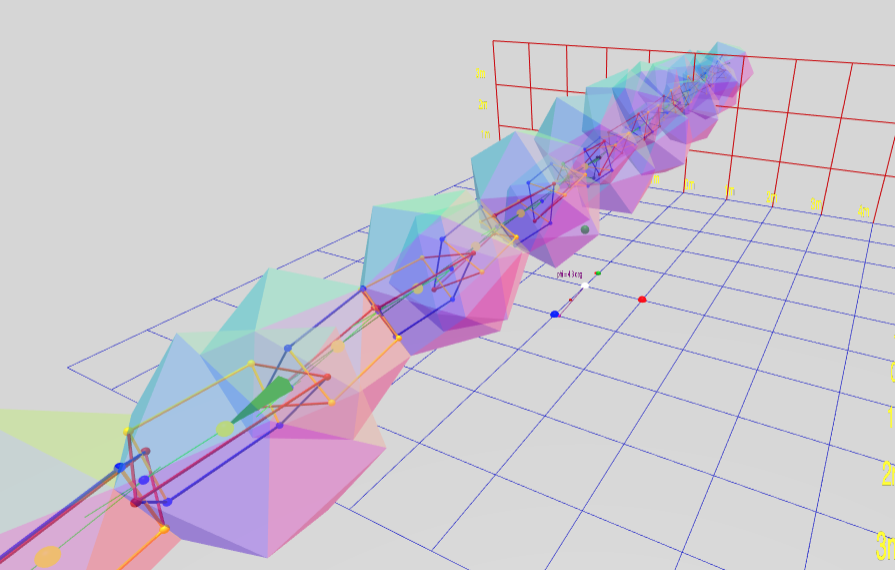
\includegraphics[width=0.40\textwidth]{figures/Planar.png}
     \caption{Quasi-planar icosahelix}
  \label{fig:quasiplanar}
\end{figure}
\item ``Two Strands'' (Figure \ref{fig:twostrands})is similar to the ``Dodecadoubler'' but even more
  visually striking. It is reminiscent of a depictions of a DNA double
  helix.
\begin{figure}
     \centering
     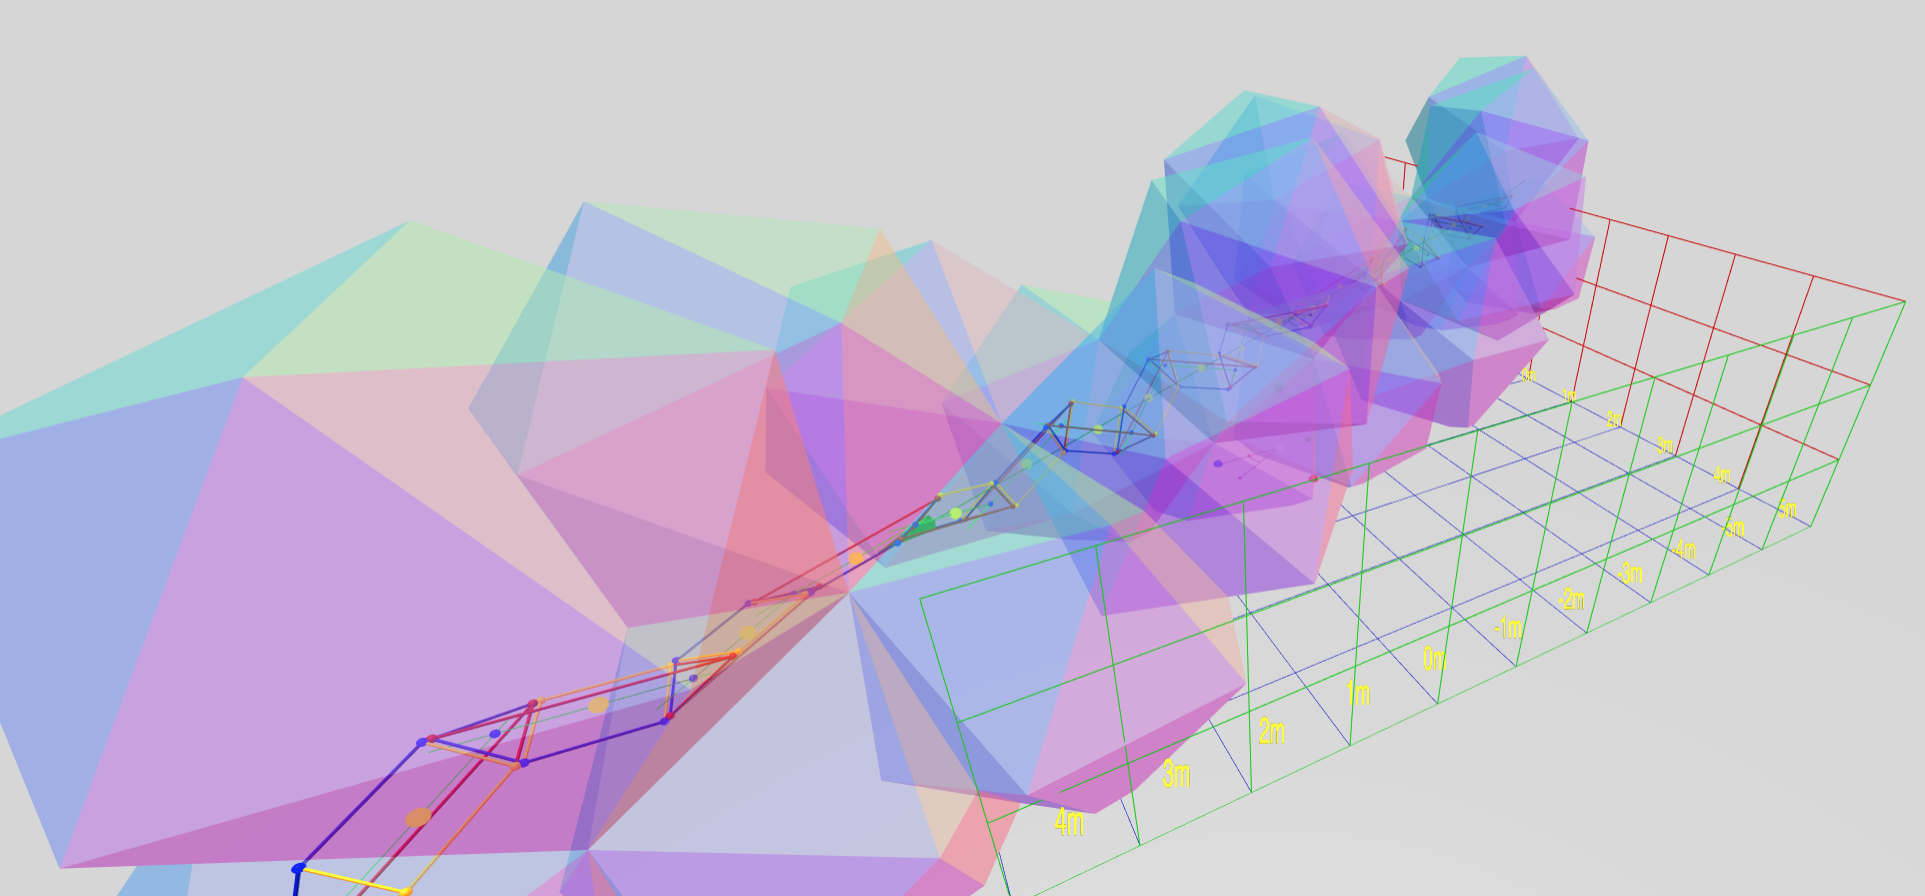
\includegraphics[width=0.40\textwidth]{figures/TwoStrands.png}
     \caption{Two Strands}
  \label{fig:twostrands}
\end{figure}
\item ``The Wheel'' (Figure \ref{fig:thewheel}) resembles a modern car tire
  in proportions.
  All Platonic solids and indeed all shapes have torus-like
  configurations. In general they do not ``close'' perfectly; that is, there is a gap that prevents the final faces from fitting together perfectly.
  However, one could make tiny adjustement to repeated shape to close this gap.
\begin{figure}
     \centering
     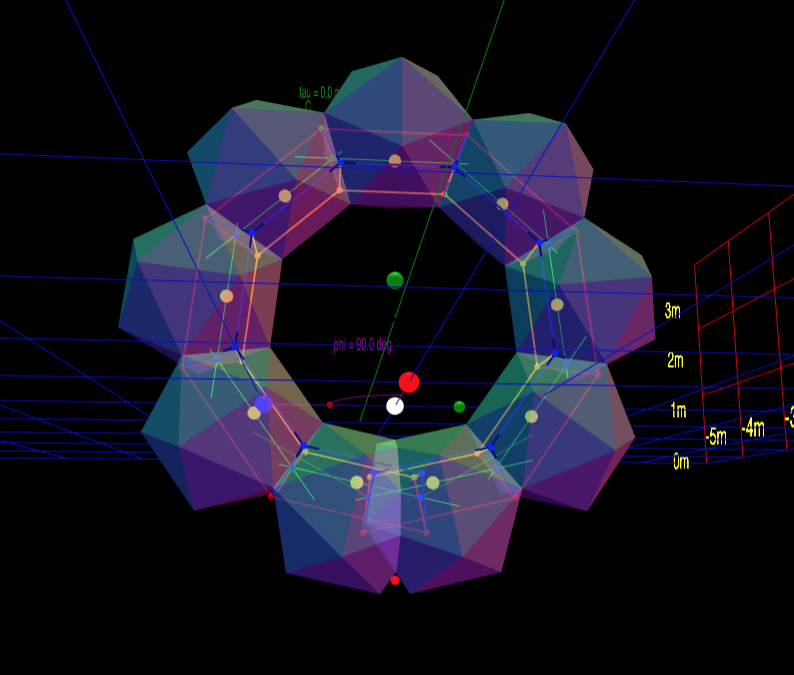
\includegraphics[width=0.40\textwidth]{figures/TheWheel.png}
     \caption{The Wheel}
  \label{fig:thewheel}
\end{figure}
\end{itemize}

\section{Future Work}

The algorithms and software described herein allow numerical calculation of the intrinsic properties of these
Platonic helices, but it would be even better to describe them in with closed-form expressions,
as Coxeter did for the Boerdijk-Coxeter tetrahelix.
The math and the algoritms are simple enough that if coded in a symbolic algebra system like Mathemtica,
or with careful work, closed-form
expressions could be produced for all the regular Platonic helices.
These would be interesting if they happen to be short; we have no reason to
believe they will be.

\section{ To Do}

\begin{itemize}
  \item Add citation to our own GitHub repo.
\item Clean up the code. 3 days
\item Go through each reference 1 day
\item Try to get list of references to the computation of a screw from an arbitrary matrix, and compare and contrast to our code. 1 day
\item Need to understand what an ``alpha coil'' protein structure is. (Done: An alpha coil is one of the most common
and studied protein forms, roughly providing distance in the protein, consisting of a helix formed by
amino acids, which tend to be cross bonded. 1 hour
\item Need to understand possibility of further simplifying specification of object.
\item Note further that Equations 7 and 8 of this paper\cite{kahn1989defining} give BETTER equations for radius $r$ and the distance $d$ than what I have so far given.
\item Need to get this paper, by hook or by crook, and probably cite:
  Note: An historical review of the theoretical development of rigid body displacements from Rodrigues parameters to the finite twist
  \url{https://www.sciencedirect.com/science/article/pii/S0094114X0500087X}
  \item Improve qualitative section, talk about toruses - 8 hours
  \item Consider better naming mechanism for faces - 4 hours
  \item Write all of the algorithms in mathematical notation
  \item Consider assigning colors to faces, which would allow for more visibility
  \end{itemize}

\section{References that need to be studied or reviewed}

This is a long, expensive book, but it may be quite relevant\cite{hyde1996language}:
\url{https://books.google.com/books?hl=en&lr=&id=1LZlSZ7ORrQC&oi=fnd&pg=PP1&ots=0hSEwJvlUB&sig=xNG9UWv_H1OXHwaOiOBJN7TW6xA#v=onepage&q&f=false}

Note: There is another long, deep book that needs to be obtained and studied\cite{sadoc2006geometrical}.
\url{https://books.google.com/books?hl=en&lr=&id=FHPlDWvz1bEC&oi=fnd&pg=PP1&ots=TsOnodavEZ&sig=HO86UUVlqRVWGqY-Tv02nb7x7NA#v=onepage&q&f=false}

\url{https://www.researchgate.net/publication/236066626_Segmented_helical_structures_formed_by_ABC_star_copolymers_in_nanopores}

This is a discussion of segmented coils in a protein structure:

\url{https://www.sciencedirect.com/science/article/pii/0022283688903701}

This talks about tuning the period of a helix inside a nanopore:

\url{https://aip.scitation.org/doi/abs/10.1063/1.4794785}

A modern helix structure protein paper:

\url{https://www.sciencedirect.com/science/article/pii/S1476927108000583}

``Local Frustration Determines Molecular and Macroscopic Helix Structures''

\url{https://pubs.acs.org/doi/abs/10.1021/jp4040503}

``Analyzing Protein Structure Using Almost Delaunay Tetrahedra''

\url{https://www.researchgate.net/profile/Alexander_Tropsha/publication/250901525_Analyzing_Protein_Structure_Using_Almost-Delaunay_Tetrahedra/links/5578584408ae75215870347c/Analyzing-Protein-Structure-Using-Almost-Delaunay-Tetrahedra.pdf}

``Simulation of Suspensions of Helical Rigid Fibers'' Y Al-Hassan : British Journal of Mathematics and Computer Science
(PDF downloaded)

``HELFIT: Helix fitting by a total least squares method'' : This needs to be studied closely!
\url{https://www.sciencedirect.com/science/article/pii/S1476927108000418}

QHELIX: A Computational Tool for the Improved Measurement of Inter-Helical Angles in Proteins
\url{https://link.springer.com/article/10.1007/s10930-007-9097-9}

Note:''On the Screw Axes and Other Special Lines Associated With Spatial Displacements of a Rigid Body''
\url{http://manufacturingscience.asmedigitalcollection.asme.org/article.aspx?articleid=1439697}

Note: An historical review of the theoretical development of rigid body displacements from Rodrigues parameters to the finite twist
\url{https://www.sciencedirect.com/science/article/pii/S0094114X0500087X}

Note: Might need to get this book.
\url{https://link.springer.com/chapter/10.1007/978-3-319-31126-5_1}


\section{Acknowledgements}

Thanks to Prof. Eric Lord for his direct communication and Mr. Robert Gatliff for his
assistance.

The enthusiasm of the participants of the 2018 Public Invention Mathathon
intitiated this work.

\bibliographystyle{unsrt}
\bibliography{shelix}

\appendix


\end{document}

\section{References Reviewed but not worth citing}

NOTE: This is a discussion of representing joint angles, it is not obvious how valuable it is:
\url{https://www.clinbiomech.com/article/S0268-0033(98)00080-1/abstract}

\url{https://www.win.tue.nl/~wstomv/publications/mathmitering-final.pdf}


\url{https://gist.github.com/peteristhegreat/3b76d5169d7b9fc1e333}

\url{https://www.sciencedirect.com/science/article/pii/S0022309307005583}


This reference is EXTREMELY IMPORTANT
\url{https://link.springer.com/article/10.1023/A:1015863923728}



This may be worth reading:
\url{https://link.springer.com/article/10.1007/PL00011063}

Some discussion of ``screw transformations''
\url{http://dergipark.gov.tr/download/article-file/56483}





\section{Mathematica Code}

\begin{verbatim}


The following math in Mathematica may be useful.

Note: Mathematica has build in Vector Angle function that can be used for alpha!!

(* c = 2 r Sin[theta/2] *)

Chord[r_,theta_] := 2 r Sin[theta/2]
 (* 1 == c^2 + d^2 *)
DZ[r_,theta_] := Sqrt[1 - Chord[r,theta]]
(* Note, this may be a problem --- Chord lenght can be diameter (2r), but I am treating it as 1 here *)
(* Some radiuses are not possible for some thetas with a length of one *)
(* Maximum radius as a function of theta *)
Mxr[theta_] := MaxValue[1 == 2 r Sin[theta/2],{r}]

Mxr[theta_] := 1/ (2  Sin[theta/2])


 Note: I should go ahead and make these functions....

(* P0 = {0, r, 0} *)
(* P1 = {r Sin[theta], r Cos[theta], d} *)
(* P2 = {r Sin[2 theta], r Cos[2 theta], 2 d} *)
(* P3 = { r Sin[3 theta], r Cos[3 theta], 3 d} *)
(* S0 = P0 - P1 *)
(* S1 = P1 - P2 *)
(* S2 = P2 - P3 *)
P[n_,r_,theta_] := { r Sin[n theta], r Cos[n theta], n DZ[r,theta]}
S[n_,r_,theta_] := P[n+1,r,theta] - P[n,r,theta]

(* Define Ps to be P symmetric; the points P0 and P1 are
symmetric in the XY plane. *)
Ps[n_,r_,theta_] :=
With[{nh = (n - (1/2))},
  { r Sin[nh theta], r Cos[nh theta], nh DZ[r,theta]}]


AlphaC[r_,theta_] := VectorAngle[S[0,r,theta],S[1,r,theta]]


f[r_, theta_] :=
 ArcCos[-1 + (r - r Cos[theta]) (-r Cos[theta] + r Cos[2 theta]) +
   4 r^2 Sin[theta/2]^2 -
   r Sin[theta] (-r Sin[theta] + r Sin[2 theta])]

Plot3D[f[r, theta]/ Degree, {r, 0, 2}, {theta, -Pi/6, Pi/6},
 AxesLabel -> Automatic]


Plot3D[AlphaC[r, theta]/ Degree, {r,0,N[Mxr[Pi]]}, {theta, 0, Pi},
 AxesLabel -> Automatic]

(*

Note: Given that we can compute $\alpha$ from $r,\theta$ in this way, one interesting thing to ask
is simply what is the minimum or maximum r (or theta) that matches an alpha. The maximum r is the
largest helix that matches, the minimum is the smallest. But with $\psi$ we will know more.
*)

PlaneNormal[a_, b_] := Normalize[Cross[a, b]]
(* Maybe psi is just theta? *)

Psi[pv0_, pv1_, v_] :=
With[{n = PlaneNormal[pv0, pv1]}, ArcSin[(n.v) /(Norm[v] Norm[n])]]

(* This is computing the angle between planes
PsiC[rx_,thetax_] :=
With[{r = rx,theta = thetax}, Evaluate[Psi[S[0,r,theta],S[1,r,theta],S[2,r,theta]]]]


Plot3D[PsiC[r, theta]/ Degree, {r, 0, N[Mxr[Pi/2]]}, {theta, 0, Pi/2},
 AxesLabel -> Automatic]

(*
Note: A strategy for computation is: given alpha, find maximum or minimum radius.
Then slow change radius until \psi if find.  However, Mathematic has optimization
built in, so we may be able to use an energy function.
*)

Enrg[alpha_,psi_,r_,theta_] := (AlphaC[r,theta] - alpha)^2 + (PsiC[r,theta] - psi)^2


(* These seem to work, but they produce rules, instead of values, what up with that? *)

Rx[alpha_,psi_] := r /. FindMinimum[Enrg[alpha,psi,r,t],{r,t}][[2]][[1]]
Tx[alpha_,psi_] := t /.  FindMinimum[Enrg[alpha,psi,r,t],{r,t}][[2]][[2]]

(* This should return 2! *)
(* Is Psi the VectorAngle of the Normals of each ABC joint? *)
Rx[AlphaC[2, Pi/20], PsiC[2, Pi/20]]
FindMinimum[Enrg[AlphaC[2, Pi/20], PsiC[2, Pi/20],r,t],{r,t}]

Unprotect[$PerformanceGoal]
$PerformanceGoal = ``Speed''

Plot3D[Rx[a,p]/Degree, {a,0,Pi/10},{p,0,Pi/10}]

(* Now that we can in theory find Rx, Tx as a function of alpha and psi,
It is important that we have a check function (or two.)
The best check would be to use a reconstruction based on transformations
of alpha and psi. I need to think about how this should be done with a
RollPitchYaw Matrix, and in what order. First you by \alpha, then you rotate by \psi.
I think we are doing ``Pitch, Roll, Yaw''. First we Pitch by \alpha, then
we Roll into the plane of the joint, then we yaw by \psi.
In fact what we are trying to do is to fly a little airplane in a helical course.
``Pitch down by alpha'', ``Yaw by psi'', ``roll so that we are perpendicular
to the the plane of the last joint''.  Maybe we never need to the roll component.
I want intrinsic angle rotation (by the definition.) We do seem to have a mobile
frame of reference.
So in fact I want EulerMatrices, not RollPitchYaw matrices.

Euluer[{\alpha,\beta,\gamma},{a,b,c}], where a,b,c = 1,2,3, let us specify those.
So we need to define how our mobile frame works. We will want $y$ to always point
``out'' of the helix, ``z'' to point along the motion'', and $x$ to be
tangential to the helix.

If we start with the intrinsic frame aligned with the extrinsic frame, repeated
transofrmations will produce a helix, but not about the $z$ axis.
We have so far described our mostion as ``rotate about y'' by $\alpha$, then
rotation about $x by $\psi$. Then our $z$ axis would be pointed in the
write direction, we would translate  by $z$, in the intrinsic frame of refrence,
and repeat.

Note, mathematica seems to have a way to render a helix, this would be very useful to me:
*)

ListPointPlot3D[
Table[Table[{t, Cos[t + s Pi/2], Sin[t + s Pi/2]}, {t, 0,
      5 Pi, .2}], {s, 4}], BoxRatios -> Automatic]

Graphics3D[
GeometricTransformation[{Hue[#/Pi], Sphere[{5, 0, 0}, 1]},
  EulerMatrix[{#, Pi/2, #}]] & /@ Range[0, 2 Pi, Pi/16]]

(* My claim is that we can somehow combine an EulerTransformation with a translation
to end up with a helix.

We can call GeometricTransoforamtion on an Euler matrix, can we pass a vector
as an object? Can we create an object of length L which is a vector
and then create a transformation?
*)

Graphics3D[Arrow[{{1, 1, 1}, {1, -1, 2}}], Axes -> True,
  AxesLabel -> {"X", "Y", "Z"}, ImageSize -> Large]

Graphics3D[
GeometricTransformation[{Hue[#/Pi],Arrow[{{1, 1, 1}, {1, -1, 2}}] },
Composition @@ {
     TranslationTransform[{1, 1, 1}],
      EulerMatrix[{0, Pi/2, #}]
}] & /@ Range[0, 2 Pi, Pi/16]]


 EulerMatrix[{Pi/15, Pi/20, 0}] [1,1,1]


 myt = TranslationTransform[{0, 0, 1}] EulerMatrix[{Pi/15, Pi/20, 0}]


 Graphics3D[{
  Opacity[1]
  , Red
  , Arrow[{{0, 0, 0}, {1, 0, 0}}]
  , Green
  , Arrow[{{0, 0, 0}, {0, 1, 0}}]
  , Blue
  , Arrow[{{0, 0, 0}, {0, 0, 1}}]
  , Opacity[0.2]
  , GeometricTransformation[Cuboid[-{1, 1, 1}/4, {1, 1, 1}/4],
   Composition @@ {
     RotationTransform[Pi/4, {0, 0, 1}]
     , TranslationTransform[{1, 1, 1}]
     }
   ]
 }]

 Graphics3D[{
  Opacity[1]
  , Red
  , Arrow[{{0, 0, 0}, {1, 0, 0}}]
  , Green
  , Arrow[{{0, 0, 0}, {0, 1, 0}}]
  , Blue
  , Arrow[{{0, 0, 0}, {0, 0, 1}}]
  , Opacity[0.2]
  , GeometricTransformation[Cuboid[-{1, 1, 1}/4, {1, 1, 1}/4],
    Composition @@ {
       RotationTransform[Pi/15,{0,1,2}],
     , TranslationTransform[{1, 1, 1}]
     }
   ]  & /@ Range[0, 5, 1]
 }]


 Graphics3D[
   GeometricTransformation[{Hue[#/Pi],Arrow[{{1, 1, 1}, {1, -1, 2}}] },
       Composition @@ {
       RotationTransform[Pi/15,{0,1,2}],
     , TranslationTransform[{1, 1, 1}]
     }
 ]]


 Composition @@ {
     RotationTransform[Pi/4, {0, 0, 1}]
     , TranslationTransform[{1, 1, 1}]
 }

 Graphics3D[

  (GeometricTransformation[Cuboid[-{1, 1, 1}/4, {1, 1, 1}/4],
   Composition @@ {RotationTransform[Pi/4, {0, 0, #}],
     TranslationTransform[{1, 1, #}]}]) & Range[3]

 ]

double[x_] := 2 x

Nest[double,#,4] & Range[3]

(* Now, what we really want to do here, is  construct
a transform out of \alpha, \pi, ending up with the arrows head to tail
*)

Clear[ComposeN]
ComposeN[0] = ScalingTransform[{1,1,1}]
ComposeN[1] = Composition @@ {
  RotationTransform[ Pi/6, {0, 1, 0}],
  Composition @@ {
    TranslationTransform[{1, 1, 1}],
    RotationTransform[ Pi/6, {0, 0, 1}]
  }
}

ComposeN[n_] :=  Composition[ComposeN[Floor[n/2]],ComposeN[Ceiling[n/2]]]


 myarrows =
 Table[
   GeometricTransformation[{
     Arrow[{{0, 0, 0}, {0, 0, 2}}],
     Arrow[{{0, 0, 0}, {0,1/2, 0}}]},
     ComposeN[i]
   ],{i,1,10}
   ]

 Graphics3D[myarrows]


 (* I think to do what I want, I need to do my own transformationns. *)
 (* An object is a vector and an upvector.
 The 0th object is a z-aligned vector starting at the origin, with a y upvector.
 The n+1th object is:
 A) Take the nth object (AB), find the head B of the vector.
 B) Create a vector of length N pointing in the same direction as the nth object.
 C) Translate it along the nth object to the head.
 D) Relative to
 E) Rotate it in the AB coordinate frame in the Y direction by Alpha.
 F) Rotate it in the X direction by Psi.
 G) Apply these same arguments to the up Vector.

Note that Mathematica has powerful RotationMatrix functions built in to which
 we can use the Nth vectors as input, to rotate in a plane. So in this sense
 we may actually be able to accomplish this.
*)

(* I'm going to try to use F to mean the nth object. *)
(* We will make the first to points computed from the Helix *)
F[0,alpha_,psi_,init_] := init

(* We are forced to pass the initial object in as a starting point *)
F[n_,alpha_,psi_,init_] :=
  With[{Prev = F[n-1,alpha,psi,init]},
      With[{
          A = Part[Prev,1], B = Part[Prev,2], U = Part[Prev,3]},
        With[{BA = B-A, UA = U-A},
        (* now we want to contruct the parts of P_n *)
        Module[{NA,NB,NU,RA,RP,NV},
          NA = B;
          V = BA;
          (* This is in theory spanned by BA, UA *)
          RA = RotationMatrix[alpha,{BA,UA}];
          RP = RotationMatrix[psi,BA];
          NB = RP.RA.V;
          NU = RP.RA.UA;
          NB = NB + B;
          NU = NU + B;
          {NA,NB,NU}
    ]
  ]]]]


  (* F requires an initial object (of three points, A, B Up.) These
  are essentially P[0],P[1], and P[0] + [0,1,0]. *)

  FTest[n_,alpha_,psi_,r_,theta_] :=
  With[{P0 = P[0,r,theta]},
    Part[F[n,alpha,psi,{P0,P[1,r,theta],P0+{0,1,0}}
      ],1]
    - P[n,r,theta]]

  FTest[1,Pi/8,0,1,0]

  FStratTest[k_,alpha_,psi_] :=
  With[
    {r = Rx[alpha,psi], t = Tx[alpha,psi], P0 = {0,0,0} },
    With[{P0 = P[0,r,t], P1 = P[1,r,t]},
      With[{init = {P0,P1,P0+{0,1,0}}},
    Print["alpha, psi, r, t ",alpha,", ",psi,", ",r,", ",t 180 / Pi];
    For[i = 0, i < k, i++,
      Print["point ",i];
      Print["P ",P[i,r,t]];
      Print["F ",Part[F[i,r,t,init],1]]
      ]
    ]
  ]]

  (* Pretty sure this is showing the r is way to small *)
  FStratTest[4, 10 Degree,10 Degree]


  (* now attempting to compute the transformation matrix
  that transforms {A,B,U},{L,N_A,N_B, Tau} into the next A,B,U.
  M = W . R . T , where W is the twist, R is the rotation,
  and T is the translation. We can test this by using a synthetic shelix to generate points and up vectors and test against that.
  *)

  (* I first need to build and test a simple Skew test.
  I want a function that yields the closest points on two skew lines,
  defined by vectors. *)

  Skew[p1_,d1_,p2_,d2_] := (* p1(2) is a point on line with direction d1(2),
  result is a vector containg C1 and C2, nearest points on those lines.
  from: https://en.wikipedia.org/wiki/Skew_lines *)
  With[{d12 = Cross[d1,d2],
      d21 = Cross[d2,d1]},
(*    Print[N[d1]]
    Print[N[d2]]
    Print[N[d12]]
    Print[N[d21]]
    Print[123123123]
    Print[N[Cross[d2,d12]]]
    Print[444444444]
    Print[N[Cross[d1,d21]]]
    Print[666666666]*)
  With[{n2 = Cross[d2,d12],
      n1 = Cross[d1,d21]},
(*    Print[555555555555]
    Print[N[n1]]
    Print[N[n2]] *)
    With[{C1 = p1 + (((p2-p1) . n2)/ (d1 . n2)) d1,
        C2 = p2 + (((p1-p2) . n1)/ (d2 . n1)) d2},
(*    Print[N[C1]]
    Print[N[C2]]
    Print[999999999999999] *)
    (* For unknown perforance reasons, I have to force evaluation to a number here *)
      {N[C1],N[C2]}]]]

  TestSkew[] :=
  With[{xp1 = {2,0,0}, xd1 = {1,0,0},
      yp1 = {1,5,1}, yd1 = {0,2,0}},
    Skew[xp1,xd1,yp1,yd1]]

  (* Now we could try a 3-point test. We take the
  first 3 points of our shelix and then compute the mid-points,
  and try to find r by treating these as skew lines with
  closes intersections. *)

  M[n_,r_,theta_] := (* midpoint of Pn-1, Pn+1 *)
  (P[n-1,r,theta]+P[n+1,r,theta])/2

  AngelBi[n_,r_,theta_] := (* unit angle bisector *)
 Normalize[M[n,r,theta] - P[n,r,theta]]

 (* This does not return the radius, it returns d, the travel *)
 (* If we made this a function of 4 points instead, then
 this would be independent of the current defintion of our
 test shelix.*)

 (* This seems to work. So if we can compute 4 points
 by virtue of the transform, we can probably compute d (z travel).
 However, the two points should let us go further. Since
 they lie on the axis plane, we can compute theta by projecting
 onto the plane normal to this line. Or just translate
 the points along this angle and then call VectorAngle.


 *)
 ComputeAxisPointsFrom4[ps_] := (* Input is a vector of four points *)
 With[{P0 = Part[ps,1],
     P1 = Part[ps,2],
     P2 = Part[ps,3],
     P3 = Part[ps,4]},
 With[{M1 = (P0+P2)/2,
     M2 = (P1+P3)/2},
   With[{B1 = Normalize[M1-P1],
       B2 = Normalize[M2-P2]},
     With[{Sk = Skew[P1,B1,P2,B2]},
       With[{C1 = Part[Sk,1],
             C2 = Part[Sk,2]},
         Print[N[VectorAngle[P1 - C1, P2 -C2]]]
         Sk
     ]]]]]

 (* I think this is supposed to return D *)
TestAxisPoint[k_,r_,theta_] :=
   With[{P0 = P[k,r,theta],
       P1 = P[k+1,r,theta],
       P2 = P[k+2,r,theta],
       P3 = P[k+3,r,theta]},
     With[{CS = ComputeAxisPointsFrom4[{P0,P1,P2,P3}]},
      Norm[Part[CS,1] - Part[CS,2]]]]

   (* IMPORTANT: This seems to be my most successful approach, the only one that is clear. *)
   (* This function returns DZ[r,theta], which seems important. *)
   (* This is the distance along the shelix axis of two points representing angle
   bisetctors. *)
  Test3PointTheory[k_,r_,theta_] :=
  With[{D0 = N[AngelBi[k,r,theta]],
      D1 = N[AngelBi[k+1,r,theta]]},
    Print[D0]
    Print[D1]
    Print[357]
    With[{CS = Skew[P[k,r,theta],D0,P[k+1,r,theta],D1]},
      Print[CS]
      Print[3333333333333]
      Norm[Part[CS,1] - Part[CS,2]]
  ]]

  (* Now beginning simple work on face diagonals *)

  Zf[w_,r_] := 1/Sqrt[1 + Tan[r]^2 + Tan[w]^2]
  Xf[w_,r_] :=
  With[{z = Zf[w,r]},
    z Tan[w]]
  Yf[w_,r_] :=
  With[{z = Zf[w,r]},
    z Tan[r]]

  TestXYZ[w_,r_] :=
  With[{ z = Zf[w,r], y = Yf[w,r], x = Xf[w,r]},
    Print N[Norm[{x,y,z}]]
    ]


  DfromOmega[L_,w_] :=
  With[{ t = Tan[w]},
    (L t) /(2Sqrt[(t^2)/4 + 1])]

  (* One way to test is to generate a synthetic shelix,
  compute rho, omega from it, and then check that this
  formular for the D from omega against this synthetic verison.
  This requires the computation of rho,omega, from r,theta *)

  (* Returns pair rho, omega (rotation about X, rotation about Y) *)
  (* This is currently wrong becasue it relies on the P0_x = P1_x,
  but I am not calculating it that way !!! *)
  (* I could compute these points and compute a rotation about Y I suppose.)
RhoOmegaFromRTheta[r_,theta_] :=
 With[{P0 = Ps[0,r,theta],
       P1 = Ps[0+1,r,theta],
       P2 = Ps[0+2,r,theta]},
   With[{a = ArcTan[Part[P1,1]/Part[P1,3]]},
     With[{rt = RotationTransform[-a,{0,1,0}]},
(*       Print[444]
       Print[N[a] 180 / Pi]
       Print[N[P1]]
       Print[N[rt[P1]]]
       Print[5555555555]
       Print[N[rt[P2]]]
       *)
     With[{v = rt[P2] - rt[P1]},
(*       Print[N[v]]  *)
       With[{x = Part[v,1],
           y = Part[v,2],
           z = Part[v,3]},
         {ArcTan[z,y],ArcTan[z,x]}
         ]]]]]


 Len[r_,theta_] := Norm[Ps[0,r,theta]-Ps[1,r,theta]]

 (* This is a check, we need to be able to compute rho and omega
 and recover the 3rd point from it. Okay, this now works. *)
 HCheck[r_,theta_] :=
 With[{ ro = RhoOmegaFromRTheta[r,theta],
   L = Len[r,theta]},
   With[{ rho = Part[ro,1], omega = Part[ro,2]},
     With[{ q = QFromRhoOmega[L,rho,omega]},
     {q Tan[omega], q Tan[rho], q}]]]


 DfromRTheta[r_,theta_] :=
 With[{ro = RhoOmegaFromRTheta[r,theta],
      L = Len[r,theta]},
   DfromOmega[L,Part[ro,2]]
   ]


 DFromLQW[L_,q_,w_] :=
 L Sin[ArcTan[Tan[w]/((L/q) - 2)]]

 ChiFromLQW[L_,q_,w_] :=
 With[{A = q Tan[w] /2,
     B = (L/2) - q},
   Print[N[A]]
   Print[N[B]]
 ArcTan[A/B]]

 TestDFromLQW[r_,theta_] :=
  With[{ ro = RhoOmegaFromRTheta[r,theta],
   L = Len[r,theta]},
   With[{ rho = Part[ro,1], omega = Part[ro,2]},
     With[{ q = QFromRhoOmega[L,rho,omega]},
       Print[N[L]]
       Print[N[q]]
       DFromLQW[L,q,omega]]]]

  (* I believe I can compute rho, omega from r,theta. I am now attempting to
  compute d from rho, omega, L, based on the projection diagrem. To debug this,
  I need to compute the points F, G, H, and check the projection diagram.
  Since I have already computed the points and a the rotation about Y which
  brings them to Z axis, this would seem to be straightforward. *)



 FGH[r_,theta_] :=
 With[{
     ro = RhoOmegaFromRTheta[r,theta],
     L = Len[r,theta],
     P0 = Ps[0,r,theta],
     P1 = Ps[0+1,r,theta],
     P2 = Ps[0+2,r,theta]},
   With[{ a = ArcTan[Part[P1,1]/Part[P1,3]],
         rho = Part[ro,1],
         omega = Part[ro,2]},
       With[{
           rt = RotationTransform[-a,{0,1,0}],
           q = QFromRhoOmega[L,rho,omega]},
       With[{ x = q Tan[omega],
           y = q Tan[rho],
           z = q },
         With[{ F = {0,0,-(L/2)},
             G = {0,0,(L/2)},
             H = {x,y,(L/2)+z},
           c = {0, Part[rt[P0],2], 0}},
           { {F,G,H},
             {rt[P0]-c,rt[P1]-c,rt[P2]-c}
             }
 ]]]]]

 (* To complete the current approach, I need to take several steps: *)
 (* Modify the code to compute $d$ from 4 arbitrary points.
 Test that this matches the current results by using a helical test pattern. *)
 (* Generate 4 points based on Rho,Omega, by using symmetry and the approach above. *)


 (* This routine generates 4 symmetric points on the Z axis matching the input values. *)
 (* To test this is sensible, I really should be able to invert it---that is,
 To find an r,theta parametrization that matches the L,rho,omega parametrization.
 Of course, in a ense, that is what we are trying to do entirely---so why not back out with my other
 computations? *)
 Generate4Points[L_,rho_,omega_] :=
 With[{
     B = {0,0,-L/2},
     C = {0,0,L/2},
     q = QFromRhoOmega[L,rho,omega]
   },
   With[{ x = q Tan[omega],
       y = q Tan[rho]},
     With[{
         A = {-x,y,-(L/2 + q)},
         D = {x,y,(L/2 + q)}},
         {A,B,C,D}
 ]]]


 Generate4PointsRTheta[r_,theta_] :=
 {Ps[-1,r,theta],Ps[0,r,theta],Ps[1,r,theta],Ps[2,r,theta]}

 (* Compute d from 4 points *)
 Bisector[X_,O_,Y_] :=
 Normalize[O - (X+Y)/2]

 (* In typical cases Skew is hanging below.
 I don't even know a mechanism by which that should be possible. *)
 ComputeDR[A_,B_,C_,D_] :=
  With[{Bb = Bisector[A,B,C],
      Cb = Bisector[B,C,D]},
    With[{CS = Skew[B,Bb,C,Cb]},
      {Norm[Part[CS,1] - Part[CS,2]],
       Norm[Part[CS,1] - B]}
  ]]

  ComputeD[A_,B_,C_,D_] :=
  Part[ComputeDR[A,B,C,D],1]


  TestComputeD[r_,theta_] :=
  With[{
      ro = RhoOmegaFromRTheta[r,theta],
      L = Len[r,theta]
    },
    With[{
        rho = Part[ro,1],
        omega = Part[ro,2]
        },
    With[{
        abcd = Generate4Points[L,rho,omega]
        },
    With[{
        A = Part[abcd,1],
        B = Part[abcd,2],
        C = Part[abcd,3],
        D = Part[abcd,4]
      },
(*      Print[N[abcd]] *)
      ComputeD[A,B,C,D] - N[DZ[r,theta]]]]]]

   TestComputeD0[r_,theta_,abcd_] :=
  With[{
      ro = RhoOmegaFromRTheta[r,theta],
      L = Len[r,theta]
    },
    With[{
        rho = Part[ro,1],
        omega = Part[ro,2]
        },
    With[{
        A = Part[abcd,1],
        B = Part[abcd,2],
        C = Part[abcd,3],
        D = Part[abcd,4]
      },
      ComputeD[A,B,C,D]]]]

  TestComputeDagainstHelix[] :=
  With[{abcd = Generate4PointsRTheta[2, Pi/10]},
    With[{
        A = Part[abcd,1],
        B = Part[abcd,2],
        C = Part[abcd,3],
        D = Part[abcd,4]
      },
      ComputeD[A,B,C,D] - DZ[2,Pi/10]]]

  TestComputeDagainstROmega[rho_,omega_] :=
  With[{abcd = Generate4Points[1, rho, omega]},
    With[{
        A = Part[abcd,1],
        B = Part[abcd,2],
        C = Part[abcd,3],
        D = Part[abcd,4]
      },
   ComputeD[A,B,C,D]]]



  (* Full test computation: Given rho,omega, compute r, theta,
  and see that it matches.
  1) Starting with r, theta, generate rho, omega, L.
  2) from rho, omega, L, generate 4 points
  3) Compute D from this.
  5) Use basic formulae to compute r,theta.
  *)

  (* Given the cord length, how do I compute R? *)


  (* Return basic helix params: r, theta, d, c *)
GetHelixParams[L_,rho_,omega_] :=
     With[{abcd = Generate4Points[L, rho, omega]},
        With[{
            A = Part[abcd,1],
            B = Part[abcd,2],
            C = Part[abcd,3],
            D = Part[abcd,4]
          },
          With[{dr = ComputeDR[A,B,C,D]},
            With[{di = Part[dr,1],
                r = Part[dr,2]},
              With[{
                  c = ChordFromLD[L,di]},
                With[{ theta2 = ThetaFromRC[r,c]},
                  {r,theta2,di,c}
                  ]]]]]]

  TestComputeDagainstROmega[rad_,theta_] :=
  With[{ L = Len[rad,theta],
      ro = RhoOmegaFromRTheta[rad,theta]},
    On[Assert];
    With[{
        rho = Part[ro,1],
        omega = Part[ro,2]},
      With[{ hp = GetHelixParams[L,rho,omega]},
        With[{ r = Part[hp,1],
            theta2 = Part[hp,2]},
          Print[theta2 180 / Pi]
          Assert[Abs[theta2 - theta] < 0.00001];
          Assert[Abs[r - rad] < 0.00001];
          Off[Assert];
          ]]]]


  (* One way to try to solve this is to fold into
  one function, then use symmetries and zeroes there
  to simplify.)

  (* This is an intermediate point with the bisector operations
  unfolded *)
  UnifiedComp0[L_,rho_,omega_] :=
  With[{
      B = {0,0,-L/2},
      C = {0,0,L/2},
      q = QFromRhoOmega[L,rho,omega]
    },
    With[{ x = q Tan[omega],
        y = q Tan[rho]},
      With[{
          A = {-x,y,-(L/2 + q)},
          D = {x,y,(L/2 + q)},
          Bb = {x/2,-y/2,(q-L)/2},
          Cb = {-x/2,-y/2,(L-q)/2}},
        With[{CS = Skew[B,Bb,C,Cb]},
            With[{
            dr = {Norm[Part[CS,1] - Part[CS,2]],
            Norm[Part[CS,1] - B]}},
              With[{di = Part[dr,1],
                  r = Part[dr,2]},
                With[{
                    c = ChordFromLD[L,di]},
                  With[{ theta2 = ThetaFromRC[r,c]},
                    {r,theta2,di,c}
      ]]]]]]]]


  (* Now I attempt to unfold the Skew *)
  UnifiedComp1[L_,rho_,omega_] :=
  With[{
      B = {0,0,-L/2},
      C = {0,0,L/2},
      q = QFromRhoOmega[L,rho,omega]
    },
    With[{ x = q Tan[omega],
        y = q Tan[rho]},
      With[{
          A = {-x,y,-(L/2 + q)},
          D = {x,y,(L/2 + q)},
          Bb = {x/2,-y/2,(q-L)/2},
          Cb = {-x/2,-y/2,(L-q)/2}},
        With[{BbXCb = N[Cross[Bb,Cb]],
            CbXBb = N[Cross[Cb,Bb]]},
          With[{n2 = N[Cross[Cb,BbXCb]],
              n1 = N[Cross[Bb,CbXBb]],
              Bbz = Part[Bb,3],
              Cbz = Part[Cb,3]},
            (* Note: C-B exist only in z dimesion! *)
         With[{CmBz = Part[C-B,3],
             BmCz = Part[B-C,3],
             n2z = Part[n2,3],
             n1z = Part[n1,3]
           },
(*           Print[555555555]
           Print[(C-B) . n2]
           Print[(CmBz)  n2z]
           Print[B-C]*)
(*          With[{CmBz = L,
                BmCz = -L
             },
             *)
            (* Note: this dot product can be replaced with a
            z multiple, since the other terms are zero *)
(*              With[{C1 = B + (((C-B) . n2)/ (Bb . n2)) Bb,
                C2 = C + (((B-C) . n1)/ (Cb . n1)) Cb},*)
              (* But that allows us to cancel out... *)
              With[{C1 = B + ((CmBz  n2z)/ (Bb . n2)) Bb,
                  C2 = C + ((BmCz  n1z)/ (Cb . n1)) Cb},
(*              With[{C1 = B + (L / Bbz ) Bb,
                    C2 = C + (-L / Cbz) Cb}, *)
(* But that can be furher simplied... *)
(*               With[{C1 = B + (2 L / (q-L) ) Bb,
                  C2 = C + (2 L / (q-L)) Cb}, *)
                    (* And then decomposed.... *)
 (*                   With[{S = 2 L / (q - L)},
                      With[{C1 = B + S Bb,
                          C2 = C + S Cb},
                        *)
                        With[{ CS =
                            {N[C1],N[C2]}},
                          With[{
                              dr = {Norm[Part[CS,1] - Part[CS,2]],
                                Norm[Part[CS,1] - B]}},
                            With[{di = Part[dr,1],
                                r = Part[dr,2]},
                              With[{
                                  c = ChordFromLD[L,di]},
                                With[{ theta2 = ThetaFromRC[r,c]},
                                  {r,theta2,di,c}
          ]]]]]]]]]]]]

N[UnifiedComp1[1, Pi/10, Pi/30]]








N[UnifiedComp2[1, Pi/10, Pi/30]]


 UnifiedComp2[L_,rho_,omega_] :=
  With[{
      B = {0,0,-L/2},
      C = {0,0,L/2},
      q = QFromRhoOmega[L,rho,omega]
    },
    With[{ x = q Tan[omega],
        y = q Tan[rho]},
      With[{
          A = {-x,y,-(L/2 + q)},
          D = {x,y,(L/2 + q)},
          Bb = {x/2,-y/2,(q-L)/2},
          Cb = {-x/2,-y/2,-(q-L)/2}},
        With[{BbXCb = Cross[Bb,Cb],
            CbXBb = Cross[Cb,Bb]},
          With[{n2 =   Cross[Cb,BbXCb],
              n1 =  Cross[Bb,CbXBb]
            },
            With[{
             n2z = Part[n2,3],
             n1z = Part[n1,3]
              },
              With[{C1 = B + ((L  n2z)/ (Bb . n2)) Bb,
                  C2 = C + ((-L  n1z)/ (Cb . n1)) Cb},
                          With[{
                              dr = {Norm[C1 - C2],
                                Norm[C1 - B]}},
                            With[{di = Part[dr,1],
                                r = Part[dr,2]},
                              With[{
                                  c = ChordFromLD[L,di]},
                                With[{ theta2 = ThetaFromRC[r,c]},
                                  {r,theta2,di,c}
          ]]]]]]]]]]]


  UnifiedComp3[L_,rho_,omega_] :=
  With[{
      B = {0,0,-L/2},
      C = {0,0,L/2},
      q = QFromRhoOmega[L,rho,omega]
    },
    With[{ x = q Tan[omega],
        y = q Tan[rho]},
      With[{
          A = {-x,y,-(L/2 + q)},
          D = {x,y,(L/2 + q)},
          (* Apparently we can take out the fact of 1/2 (1/8) here *)
          Bb = {x,-y,(q-L)},
          Cb = {-x,-y,-(q-L)}},
        With[{BbXCb = Cross[Bb,Cb],
            CbXBb = Cross[Cb,Bb]},
          With[{n2 =   Cross[Cb,BbXCb],
              n1 =   Cross[Bb,CbXBb]
            },
            With[{
             n2z = Part[n2,3],
             n1z = Part[n1,3]
              },
              With[{Bn2 = n2z / (Bb . n2),
                    Cn1 = n1z / (Cb . n1)},
              With[{C1 = B + (L  Bn2) Bb,
                  C2 = C + (-L  Cn1) Cb},
                          With[{
                              dr = {Norm[C1 - C2],
                                Norm[C1 - B]}},
                            With[{di = Part[dr,1],
                                r = Part[dr,2]},
                              With[{
                                  c = ChordFromLD[L,di]},
                                With[{ theta2 = ThetaFromRC[r,c]},
                                  {r,theta2,di,c}
  ]]]]]]]]]]]]


N[UnifiedComp3[1, Pi/10, Pi/30]]

 UnifiedComp4[L_,rho_,omega_] :=
  With[{
      B = {0,0,-L/2},
      C = {0,0,L/2},
      q = QFromRhoOmega[L,rho,omega]
    },
    With[{ x = q Tan[omega],
        y = q Tan[rho]},
      With[{
          A = {-x,y,-(L/2 + q)},
          D = {x,y,(L/2 + q)},
          (* Apparently we can take out the fact of 1/2 (1/8) here *)
          Bb = {x,-y,(q-L)},
          Cb = {-x,-y,-(q-L)}},
        With[{BbXCb = Cross[Bb,Cb],
            CbXBb = Cross[Cb,Bb]},
          With[{n2 =   Cross[Cb,BbXCb]
(*              n1 =   Cross[Bb,CbXBb] *)
            },
            With[{
             n2z = Part[n2,3]
(*             n1z = Part[n1,3] *)
              },
              With[{Bn2 = n2z / (Bb . n2)
                (*  Cn1 = n1z / (Cb . n1) *)
                },
              With[{C1 = B + (L  Bn2) Bb
(*                  C2 = C + (-L  Cn1) Cb *)
                },
                (* A Key point -- C1.y = C2.y, and C2.x = - C2.x, and C2.z = - C2.z *)
                (* This should simplify the norming operation below! *)
                (* I this case the norm depends only on x and z:
                With[{A = {a, b, c},
         B = {-a, b, -c}},
                  Norm[A - B]] => 2Sqrt[a^2 + c^2] *)
                (* So, in the first place, don't compute C2! *)
                          With[{
                              di = 2Sqrt[Part[C1,1]^2 + Part[C1,3]^2],
                              r =   Norm[(L  Bn2) Bb]},
                              With[{
                                  c = ChordFromLD[L,di]},
                                With[{ theta2 = ThetaFromRC[r,c]},
                                  {r,theta2,di,c}
  ]]]]]]]]]]




N[UnifiedComp4[1, Pi/10, Pi/30]]



 QFromRhoOmega[L_,rho_,omega_] :=
 L/Sqrt[1+Tan[rho]^2+Tan[omega]^2]

  ChordFromLD[L_,D_] := Sqrt[L^2 - D^2]
  ThetaFromRC[R_,C_] :=
  2 ArcSin[C/(2R)]

 UnifiedComp5[L_,rho_,omega_] :=
  With[{
      B = {0,0,-L/2},
      q = QFromRhoOmega[L,rho,omega]
    },
    With[{ x = q Tan[omega],
        y = q Tan[rho],
      u = q - L},
      With[{
          A = {-x,y,-(L/2 + q)},
          D = {x,y,(L/2 + q)},
          (* We have removed a factor of 1/2 (1/8) here *)
          Bb = {x,-y,u},
          Cb = {-x,-y,-u}},
        With[{n2 =   Cross[Cb,Cross[Bb,Cb]]
          },
            With[{
             n2z = Part[n2,3]
              },
              With[{Bn2 = n2z / (Bb . n2)
                },
                With[{LBn2 = L Bn2},
              With[{C1 = B + LBn2 Bb
                },
                With[{
                    di = 2Sqrt[Part[C1,1]^2 + Part[C1,3]^2],
                    r =   Abs[LBn2] Norm[ Bb]},
                  With[{
                      c = ChordFromLD[L,di]},
                    With[{ theta2 = ThetaFromRC[r,c]},
                      {r,theta2,di,c}
  ]]]]]]]]]]]



  (* Note, possibly this would be better done with C,D, or A,B *)
  (* Also, this neither takes nor returns tau, so it must be making an assumption *)
  (* How do we compute tau from this? tau should be computed from the points C1, D
  As teh change in the upvector. *)
UnifiedCompTwoPoints[L_,B_,D_] :=
With[{q = D[[3]] - L/2,
      x = D[[1]],
      y = D[[2]]},
    With[{u = q - L},
      With[{Bb = {x,-y,u},
          Cb = {-x,-y,-u}},
(* N2 normal of the plane normal to the axis and Cb, along which the skew alogirthm moves. *)
        With[{n2 =   Cross[Cb,Cross[Bb,Cb]]
          },
            With[{
             n2z = Part[n2,3]
              },
              With[{Bn2 = n2z / (Bb . n2)
                },
                With[{LBn2 = L Bn2},
              With[{C1 = B + LBn2 Bb
                },
                With[{
                    di = 2Sqrt[Part[C1,1]^2 + Part[C1,3]^2],
                    r =   Abs[LBn2] Norm[ Bb]},
                  With[{
                      c = ChordFromLD[L,di]},
                    With[{ theta2 = ThetaFromRC[r,c]},
                    Print[N[{r,theta2,di,c,C1}]];
                      {r,theta2,di,c,C1}
  ]]]]]]]]]]]

(* Now attempting to test the hypotheis that d = (P2 - P1 dot (V1 x V2) *)
Kahn[L_,B_,D_] :=
With[{q = D[[3]] - L/2,
      x = D[[1]],
      y = D[[2]]},
    With[{u = q - L,
        C = {0,0,L/2}},
      With[{Bb = {x,-y,u}, (* This is the B bisector *)
      Cb = {-x,-y,-u}},(* This is the C bisector *)
          With[{H = Cross[Bb,Cb]},
          With[{
(* I am very confused by this. I don't know that is right. *)
          dtravel = (C - B) . Normalize[H],
(* n2 is from the skew algorithm, it is the normal for the plane containing Cb
and perpendicular to helix axis *)
          n2 =   Cross[Cb,H]
          },
(* It is unclear why this should be negative, need a way of determining that. *)
          With[{phi = -ArcCos[dtravel/L]},
          With[{
          (* Not sure how to compute the signs here *)
          Baxx = Sin[phi] dtravel/2,
          Bazz = -Cos[phi] dtravel/2
          },
            With[{
            Bayy =  Bb[[2]] (Baxx/Bb[[1]]),
             n2z = Part[n2,3]
              },
(* This (n2z) is really the factor (C - B) . n2, but we know that is zero exept for z *)
(* {0,0,n2z} is the projection of (C-B) onto n2 *)
              With[{
              Ba = {Baxx,Bayy,Bazz},

              Bn2 = n2z / (Bb . n2),
(* This is an alternative factor for clarity, but we know only the z matters. *)
              AF = ((C - B) . n2)/(Bb . n2)
                },
                With[{LBn2 = L Bn2},
(* C1 is the axial projection of C (Except I now think NOT!) *)
              With[{
              Ca = {-Ba[[1]],Ba[[2]],-Ba[[3]]},
              B1 = B + LBn2 Bb,
              B1x = B + AF Bb
                },
Print[8888];
Print[{B1,B1x,Ba}];
Print[{Ca}];
Print[{Norm[Ba-B],Norm[Ca-C]}];
(* Print[{AF,LBn2,s}]; *)
                With[{
(*                    di = 2Sqrt[Part[B1,1]^2 + Part[B1,3]^2],
                    r =   Abs[LBn2] Norm[ Bb],*)
                    r = Norm[Ba-B]},
                    Print[{dtravel}];
                    Print[2222];
                  With[{
                      c = ChordFromLD[L,dtravel]},
                    With[{ theta2 = ThetaFromRC[r,c]},
                    Print[{r,r}];
                    Print[N[{r,theta2,dtravel,c}]];
                      {r,theta2,dtravel,c}
  ]]]]]]]]]]]]]]


(* From _Mastering Mathematica_, by John W. Gray \cite{gray1998mastering}*)
Attributes[withRec ] = {HoldFirst};
withRec[x_, exprl_, expr2_] :=
 FixedPoint[With[{x = exprl}, #] &, expr2]

(* Try this in the morning:
Something like: Block[{}, Begin[Unique[]<>"`"]; do-whatever; End[]; return-value]
Any symbols defined in do-whatever are put in the new context created by Begin, and the context is removed before the block ends.
*)

(* Phi is the amount of rotation needed to make the segment
align with the axis. I think that makes this negated, but we
may have to do a quadrant test. *)
(* Same as: phi = VectorAngle[{H[[1]],0,H[[3]]},{0,0,1}]} *)

ChordFromLDaxis[L_,Da_] := Sqrt[L^2 - Da^2]
RotationFromRadiusChord[R_,C_] := 2 ArcSin[C/(2R)]
PointAxis[L_,{x_,y_,z_}] := Block[{A, B, C, D, Cb, Bb, H,
                                  Bax, Bay, Baz, Ba,
                                  r, theta, da, c, phi},
  D = {x,y,z};
  A = {-x, y, -z};
  B = {0, 0, -L/2};
  C = {0, 0, L/2};
  Cb = (B+D)/2 - C;
  Bb = (A+C)/2 - B;
  H = Normalize[Cross[Bb,Cb]];
  da = (C - B) . Normalize[H];
  phi = ArcCos[da/L];
  Bax = Sin[phi] da / 2;
  Baz = -Cos[phi] da / 2;
  Bay = Bb[[2]] (Bax / Bb[[1]]);
  Ba = {Bax,Bay,Baz};
  r = Norm[Ba - B];
  c = ChordFromLDaxis[L,da];
  theta = RotationFromRadiusChord[r,c];
  {r,theta,da,c,phi,H}
]





(* This does not seem to take tau into effect. Unified Comp needs to return tau *)
UnifiedComp7[L_,rho_,omega_] :=
  With[{
      B = {0,0,-L/2},
      q = QFromRhoOmega[L,rho,omega]
    },
    With[{ x = q Tan[omega],
        y = q Tan[rho],
      u = q - L},
      With[{
          D = {x,y,(L/2 + q)}
        },
        Kahn[L,B,D]]]]


  N[UnifiedComp5[1, Pi/10, Pi/30]]
  N[UnifiedComp7[1, Pi/10, Pi/30]]


Plot3D[Part[UnifiedComp5[1,rho,omega],3],{rho,0,Pi/4},{omega,0,Pi/4},AxesLabel->{rho, omega}]

Plot3D[Part[UnifiedComp5[1,rho,omega],1],{rho,0,Pi/2},{omega,0,Pi/30},AxesLabel->{rho, omega}]

Plot[Part[UnifiedComp5[1,rho,0],1],{rho,0,Pi/2},AxesLabel->{rho}]

Plot[Part[UnifiedComp5[1,Pi/30,omega],1],{omega,0,Pi/2},AxesLabel->{omega}]



(* In this section, I am purely attempting to work out the
coordinates of the two face-to-face tetrahedra in order to
compute rho, omega in this platonic case. *)

(* This is all wrong because the centroid to centroid distance is actually 1/3 *)
(* These are values for a regular tetrahedron, I think. *)
(* These numbers are wrong, I think... *)
alphaA = 0;
alphaB = 0;
betaA = ArcTan[Sqrt[2]/2];
betaB = ArcTan[Sqrt[2]/2];


tau = 2 Pi / 3;

(* I now believe these are wrong, and the approach is probably
wrong. Instead we need to use Rodrigues' rule, rotate by tau,
and get the resulting unit vector back and apply simple trig
to it to get omega and rho. Note this also raises the
question that it might be better to consider the face angles
as unit vectors in the first place, but you still have to
rotate them. However, possibly unfolding the definition of rho and
omega as unit vectors will let us come closer to a formula.
We will, however, write this as rotating a vector of length L,
becasue that way a valuable point will be produced for our
compuation later. *)

(* I may not need this with built in Mathematica stuff. *)
vRot[k_,v_,theta_] := v Cos[theta] + Cross[k,v] Sin[theta]
+ k (k . v)(1 - Cos[theta])

vRotM[k_,theta_] :=
With[{ x = Part[k,1],
    y = Part[k,2],
    z = Part[k,3]},
  With[{C = {
        {0, -z, y},
        {z, 0, -x},
        {-y,x, 0}
    }},
    Print[C // MatrixForm];
    Print[(1 - Cos[theta])C^2 // MatrixForm];
    Print[IdentityMatrix[3] + (1 - Cos[theta])C^2 // MatrixForm];
    Print[IdentityMatrix[3] + (Sin[theta] C)+ (1 - Cos[theta])C^2 // MatrixForm];
    IdentityMatrix[3] + (Sin[theta] C) + (1 - Cos[theta]) C^2]]

vRotAux[k_,v_,theta_] :=
vRotM[k,theta].v

(* NOTE: This is incorrect, the vector v must be rotated into
k. I is the opposite of k (if symmetric) but must be rotated. *)
testvRot[tau_] :=
With[{alphaA = 0,
    alphaB = 0,
    betaA = -ArcTan[Sqrt[2]/2],
    betaB = ArcTan[Sqrt[2]/2],
    L = 1
  },
  With[{k = Normalize[{Sin[alphaB],Sin[betaB],Cos[betaB]}]},
    With[{
      v = Normalize[-L {Sin[alphaA],Sin[betaA],Cos[betaA]} + k]
    },
    Print[k];
    Print[Norm[k]];
    Print[v];
    Print[Norm[v]];
    With[{ rt = RotationTransform[tau,k]},
      With[{
          (*  vr = vRot[k,v,tau] *)
          vr = rt[v]
        },
      Print[N[vr]];
      Print[Norm[vr]];
      Print[N[Normalize[vr]]];
      With[{ x = Part[vr,1],
          y = Part[vr,2],
          z = Part[vr,3]},
        With[{ ro =
            (* Warning: Mathematic uses x,y order here, Javascript other *)
            { ArcTan[z,y],ArcTan[z,x]}},
          Print[N[ro 180 / Pi]];
          ro]]]]]]]




N[ArcTan[Sqrt[2]/2]]


(* Starting new work here. This is an attempt to compute
the point A (and thereby D) from NB and NC (normal vectors)
and tau (and L). This is based on my new understand that
we can compute a vector to be rotated.

I hope to test this with both regular regular objects,
but in the end with the regular tetrahedron, for which
we have a known solution (via Javascript work.)

Variables:

NB = Vector normal of the face containing B
NC = Vector normal of the face containg C
L = distance between B and C
tau = the twist

PA = the projection of BA onto the vector NB
R = The up-pointing rejection of BA onto NB. (perpendicular)
delta = angle between NC and the axis
gamma = angle between the XZ plane and the NB vector.

V0 = Vector to be rotated

AfromParams[v0,taux,NB] -- a function to compute A

V0fromLNB[L,NB,delta]

TestAWith225s[] = test AfromParams with faces cut and 22.5 degrees

*)

AngleWithXZ[v_] :=
VectorAngle[{v[[1]],0,v[[3]]},v]

(* I now believe this should be done with a rotation.
V0 is a rotation of NB vector by delta in the pure
up direction (that is, in the ZY plane about {1,0,0} *)
V0fromLNB[L_,NB_,NC_,delta_] :=
With[{k = Normalize[NB],
    rt = RotationTransform[-delta,{1,0,0}]},
  With[{ v0 = L Normalize[rt[NB]]},
    v0]
  ]

(* Apparently I am treating tau as the rotation about the normal. *)
ADirFromParam[L_,v0_,tau_,NB_] :=
With[{k = Normalize[NB]},
  With[{ rt = RotationTransform[tau,k]},
    L  Normalize[rt[v0]]]]

ComputeBalancingRotation[NB_,NC_] :=
(* our stategy will be to project on the XY plane,
and then compute the midpoint vector *)
With[{ NBN = Normalize[NB],
    NCN = Normalize[NC]},
  With[{Bp = {NBN[[1]],NBN[[2]]},
      Cp = {NCN[[1]],NCN[[2]]}},
    With[{ ba = ArcTan[Bp[[1]],Bp[[2]]],
           ca = ArcTan[Cp[[1]],Cp[[2]]]},
    With[{m = Bp+Cp},
      With[{mn = m / 2},
        (* We want to return the angle that makes the negative of this vector point up *)
        With[{theta = -(ba+ca)/2 + -Pi/2 },
          With[{
              (*              rt = RotationTransform[{{mn[[1]],mn[[2]],0},{0,-1,0}}] *)
              rt = RotationTransform[-theta,{0,0,-1}]
            },
            With[{ Br = rt[NB],
                Cr = rt[NC]},
              Print[N[{theta,Br,Cr}]];
              {theta,Br,Cr}
      ]]]]]]]]

TestComputeBalancingRotation[] :=
With[{C = {1,1/2,1},
    B = {-1/2,-1,-1}},
  With[{res = ComputeBalancingRotation[B,C]},
    Print[res];
    With[{ theta = res[[1]],
        Br = res[[2]],
        Cr = res[[3]]},
      With[{Bp = Normalize[{Br[[1]],Br[[2]]}],
          Cp = Normalize[{Cr[[1]],Cr[[2]]}]},
        Print[8888888];
        Print[N[Bp]];
        Print[N[Cp]];
        Assert[N[Bp[[1]]] == -N[Cp[[1]]]];
        Assert[Bp[[2]] < 0];
        Assert[Cp[[2]] < 0];
        res
  ]]]]

(* This is untested, I am not sure what will happend here *)
TestComputeBalancingRotation1[] :=
With[{C = {0,0.3,1},
    B = {0,-0.2,-1}},
  With[{res = ComputeBalancingRotation[B,C]},
    Print[res];
    With[{ theta = res[[1]],
        Br = res[[2]],
        Cr = res[[3]]},
      With[{Bp = Normalize[{Br[[1]],Br[[2]]}],
          Cp = Normalize[{Cr[[1]],Cr[[2]]}]},
        Print[8888888];
        Print[N[Bp]];
        Print[N[Cp]];
        Assert[N[Bp[[1]]] == -N[Cp[[1]]]];
        Assert[Bp[[2]] < 0];
        Assert[Cp[[2]] < 0];
        res
  ]]]]

TestComputeBalancingRotation2[] :=
With[{C = {1,3/4,1},
    B = {1,0,-1}},
  With[{res = ComputeBalancingRotation[B,C]},
    Print[N[res]];
    With[{ theta = res[[1]],
        Br = res[[2]],
        Cr = res[[3]]},
      With[{Bp = Normalize[{Br[[1]],Br[[2]]}],
          Cp = Normalize[{Cr[[1]],Cr[[2]]}]},
         Print[8888888];
        Print[N[Bp]];
        Print[N[Cp]];
        Assert[N[Bp[[1]]] == -N[Cp[[1]]]];
        Assert[N[Bp[[1]]] == -N[Cp[[1]]]];
        Assert[Bp[[2]] < 0];
        Assert[Cp[[2]] < 0];
        res
  ]]]]



TestComputeBalancingRotation3[] :=
With[{
    L0 = 1,
    tetAngle = ArcTan[Sqrt[2]/2],
    (* Rotation by an aribitraty amount should give us the same number. *)
    testRot = Pi/4
  },
  With[{ rt = RotationTransform[testRot,{0,0,1}]},
    With[{
        plainB = {0,-Sin[tetAngle],-Cos[tetAngle]},
        plainC = {0,-Sin[tetAngle],Cos[tetAngle]},
        tau = 2 Pi /3
      },
   With[{C = rt[plainB],
       B = rt[plainC]},
  With[{res = ComputeBalancingRotation[B,C]},
    Print[N[res]];
    With[{ theta = res[[1]],
        Br = res[[2]],
        Cr = res[[3]]},
      With[{Bp = Normalize[{Br[[1]],Br[[2]]}],
          Cp = Normalize[{Cr[[1]],Cr[[2]]}]},
         Print[8888888];
        Print[N[Bp]];
        Print[N[Cp]];
        Assert[N[Bp[[1]]] == -N[Cp[[1]]]];
        Assert[N[Bp[[1]]] == -N[Cp[[1]]]];
        Assert[Bp[[2]] < 0];
        Assert[Cp[[2]] < 0];
        res
  ]]]]]]]

(* Warning: I may not have the sign of this correct. *)
AfromLtauNBNC[L_,tau_,NBunb_,NCunb_] :=
With[{ res = ComputeBalancingRotation[NBunb,NCunb]},
  With[{NB = res[[2]],
    NC = res[[3]]},
    With[{delta = VectorAngle[{0,0,1},NC]},
      With[{v0 = V0fromLNB[L,NB,NC,delta]},
        Assert[N[Norm[v0]] == L];
        With[{ Ad = ADirFromParam[L,v0,tau,NB],
            B = {0,0,-L/2}},
          Assert[Abs[Norm[Ad] -L ] < 0.00001];
          Ad + B]]]]]

(* For testing, I create a block of size 1
with NB and NC based on half of a 45 degree angle. *)
(* I need to write a function that takes two face normals,
and computes the balancing of them, returning two new normals
that are balanced around the up vector. Then I need
to test that the same point is computed from both directions
even when we have unbalanced normals. *)

TestAfromLtauNBNC[tau_] :=
With[{
    L0 = 1,
    NB0 = {0,-Sin[Pi/8],-Cos[Pi/8]},
    NC0 = {0,-Sin[Pi/8],Cos[Pi/8]},
    tetAngle = ArcTan[Sqrt[2]/2]},
  With[{
      NB1 = {0,-Sin[tetAngle],-Cos[tetAngle]},
      NC1 = {0,-Sin[tetAngle],Cos[tetAngle]},
      B = {0,0,-L/2}
    },
    With[{
        AA = AfromLtauNBNC[L0,tau,NB1,NC1]
      },
      AA
  ]]]

(* I need to write a test that sends the face normals
into UnifiedComp. Probably it would be better
to separate out a version of UnifiedComp that takes
points (the rho/omega version can implement that. *)


On[Assert];

TestRegularTets[] :=
With[{
    L0 = 1/3,
    tetAngle = ArcTan[Sqrt[2]/2]},
  With[{
    NB1 = {0,-Sin[tetAngle],-Cos[tetAngle]},
    NC1 = {0,-Sin[tetAngle],Cos[tetAngle]},
    tau = 2 Pi /3
    },
    With[{
        A = AfromLtauNBNC[L0,tau,NB1,NC1]},
      Print[N[A]];
      With[{ B = {0,0,-L0/2},
          D = {-A[[1]],A[[2]],-A[[3]]}
        },
        With[{ res = UnifiedCompTwoPoints[L0,B,D],
            theta = ArcCos[-2/3]},
          Assert[Abs[res[[2]] - theta] < 0.00001];
]]]]]

TestRegularTets1[] :=
With[{
    L0 = 1/3,
    tetAngle = ArcTan[Sqrt[2]/2]},
  With[{
    NB1 = {0,-Sin[tetAngle],-Cos[tetAngle]},
    NC1 = {0,-Sin[tetAngle],Cos[tetAngle]},
    tau = 2 Pi /3
    },
    With[{
        A = AfromLtauNBNC[L0,tau,NB1,NC1]},
      With[{ B = {0,0,-L0/2},
          D = {-A[[1]],A[[2]],-A[[3]]}
        },
        With[{res = PointAxis[L0,D],
            thetaExp = ArcCos[-2/3]},
            Block[{r,theta,da,c,phi,H},
            {r,theta,da,c,phi,H} = res;
            Print[{r,theta,da,c,phi}];
            Print[N[{r,theta 180 / Pi,da,c, phi 180 / Pi}]];
          Assert[Abs[res[[2]] - thetaExp] < 0.00001]
]]]]]]

TestRegularTets2[] :=
With[{
    L0 = 1,
    tetAngle = ArcTan[Sqrt[2]/2],
    (* Rotation by an aribitraty amount should give us the same number. *)
    testRot = Pi/5
  },
  With[{ rt = RotationTransform[testRot,{0,0,1}]},
    With[{
        plainB = {0,-Sin[tetAngle],-Cos[tetAngle]},
        plainC = {0,-Sin[tetAngle],Cos[tetAngle]},
        tau = 2 Pi /3
      },
      With[{ NB1 = rt[plainB],
      NC1 = rt[plainC]},
      Print[{plainB,plainC}];
      Print[{NB1,NC1}];
      With[{
          A = AfromLtauNBNC[L0,tau,NB1,NC1]},
      Print[N[A]];
        With[{ B = {0,0,-L0/2},
            D = {-A[[1]],A[[2]],-A[[3]]}
          },
          With[{ {r,theta,da,c,phi} = Kahn2[L0,B,D],
              theta_exp = ArcCos[-2/3]},
            Assert[Abs[theta - theta_exp] < 0.00001];
]]]]]]]


(* Trying something new *)
Clear[a,b,c,d,e,f,h,i,j,k,l,m,n,o,p,q,r,s,t,u,x,y]
Solve[{a == h x + p, b == i x + q, c == j x + r, d == l x + s, e == m x + t, f == n x + u, d^2 == (a-d)^2 + (b-e)^2 + (c-f)^2,
q == 0, t == 0, r == -u, p == -s},x]

Solve[{a == h x + p, b == i x + q, c == j x + r, d == l x + s, e == m x + t, f == n x + u, z^2 == (a-d)^2 + (b-e)^2 + (c-f)^2,
q == 0, t == 0, r == -u, p == -s},x]


Solve[{a == h x + p, b == i x + q, c == j x + r, z^2 == (a)^2 + (b)^2 + (c)^2},
,{x},Reals]

\end{verbatim}





\section{Computation of Segmented Helix}

In this section we attempt to derive formulae for $r,d,/theta$ from
the instrinsic properties of the object.

\section{Old Work}

The most easily measured relationship between the segments
is the angle $\alpha$ in the plane containing both of the segments. (If the segments are coincident and therefore
parallel $\alpha$ will be $\pi$. If $\alpha < \pi/2$, the segment ``bends backward''.
The final measure that is needed is the rotation about a member between the elements attached to it.
Let us call this angle $\psi$. That is, if you look along the axis of an object at the line
between the joints, the two members form an angle between 0 and $\pi /2$.

\begin{align*}
    A &= P(-1)  \\
    B &= P(0) \\
    C &= P(1)
\end{align*}

$A,B,C$ form an isoceles triangle that contains $\overline{AB}$ and $\overline{BC}$, and therefore the angle $\alpha$ is in
this plane. Forming the kite $ABCO$, we see that one diagonal is $r$ and the other diagonal is $2 r \sin{\theta}$, where
$y = r \sin{\theta}$ is half of this diagonal.

\begin{align*}
    y &= r \sin{\theta}  \\
    z^2 &= c^2 - y^2 \\
    z^2 &= c^2 - (r \sin{\theta})^2 \\
    q^2 + z^2 &= L^2 \\
    q &= \sqrt{L^2 - z^2} \\
    q &= \sqrt{L^2 - (c^2- (r\sin{\theta})^2)} \\
    q &= \sqrt{L^2 + (r\sin{\theta})^2 - (2r\sin{\theta/2})^2 } \\
    \sin{\alpha/2} &= q/L \\
    q &= L \sin{\alpha/2} \\
    \alpha/2 &= \arcsin{q/L} \\
    \alpha &= 2 \arcsin{\frac{\sqrt{L^2 + (r\sin{\theta})^2 -
          (2r\sin{\theta/2})^2}}
      {L}} \\
\end{align*}

Note $y$ is in the projected kite, $q$ is in the slanted kite.
Rearranging these relationships in terms of known quantites $L, \alpha, \psi$, we have:

\begin{align*}
  \sin{\alpha/2} &= q/L \\
  q &= L \sin{\alpha/2} \\
  z^2 &= L^2 - q^2 \\
  %% Now we must use \psi
  \beta &= \frac{\pi - \theta}{2} \\
  \frac{z}{c} &= \cos{\beta} \\
  c &= \frac{z}{\cos{\beta}} \\
  y^2 &= c^2 - z^2 \\
  r &= \frac{y}{\sin{\theta}} \\
  d^2 &= L^2 - c^2 \\
  \phi &= \arctan{c/d} \\
\end{align*}

I think we can compute $\psi$ from $\theta$ easily enough. The problem is going the other way.

\subsection{An alternate approach}

Rather than starting with $\alpha$ and $\psi$ as inputs, we can think of a vector $v$ that
moves in the positive $\overline Z$ direction, $\overline Z = \overline P_1 - \overline P_0$, and
the angle $\theta$ which $Z$ rotates about the $z$-axis at each step. If a rotation matrix $M$
represents rotation about and $T$ represents translation along the $z$-axis, then $P_n = (M+T)^nP_n$.


\subsection{Old Approach}


Consider a slender cylinder or prism with two faces $F_0,F_1$ cut at arbitrary angles to the axis of the cylinder.
Joining two such cylinders at the axes by placing $F_0$ angainst $F_1$ produced a joint with a difference in
angle between the axes of $\alpha$ and a rotation of the orienation of the faces about the axis of $\theta$.
Note that $\alpha$ and $\theta$ are a function of the vectors normal to the faces to be joined, but are not the same as them. $\alpha$ and $\theta$ are likely combinations of the face angles.

\begin{theorem}[Stacking Helix]
  The joints of a sequential stack of objects of length $L$ whose joints axis change by $\alpha$ and orientation rotate
  by $\theta$ are intersected by a helix of radius and pitch easily numerically computable
  from  $L,\alpha$, and $\theta$.
\end{theorem}

\begin{figure}
     \centering
     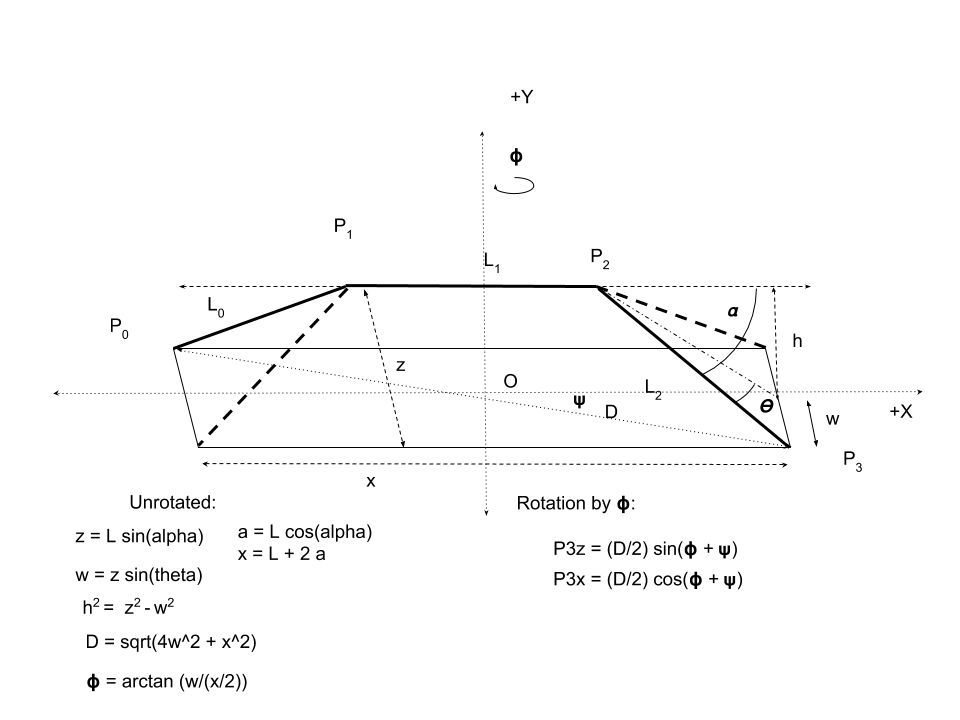
\includegraphics[width=0.95\textwidth]{figures/StackedSetup.png}
     \caption{The rotatable prism of three objects}
  \label{fig:prismdiagram}
\end{figure}

\begin{proof}

  In Figure \href{fig:prismdiagram}, let $L_i$ be the $i$th instance of the length-$L$ objects. Let $\alpha$ be the
  change in angle in the axes at a joint (the point were axes meet) measured in the plane containing the axes of both objects. (If these axes are parallel (and therefore coincident) define $\alpha$ to be 0.
  Let $\theta$ be the change in orientation relative to the axis,
  or, the half-angle formed by $L_0$ and $L_2$ when projected onto a plane normal to the axis of $L_1$.
  Without loss of generality, choose the measures of these angles in radians so that
  $0 \leq \theta < \pi/2$ and $0 \leq \alpha < \pi$.
  Take $\alpha < 0$ to mean that objects $L_0$ and $L_1$ bend away from each other,
  and $\alpha > 0$ to mean that the objects $L_0$ and $L_1$ bend toward each other.

  If $\theta = 0$ and $\alpha > 0$, the stack will form a circle-like structure or radius
  $\frac{L}{2 \sin{\frac{\alpha}{2}}}$, as shown in Section \ref{sec:2d}, where as if
  $\theta = 0$ and $\alpha < 0$, then stack will form a sawtooth-like structure.

  Note that any angle $\alpha$ is possible, if we do not concern oursleves with the self-collision
  of physical objects. $\alpha > \pi/2$ means the stack ``turns back on itself'' to some extent.

  If we arrange object $L_1$ so that its axis lies on the $x$-axis and its midpoint is at the origin,
  $L_0$ and $L_1$ extend from it symmetrically in the projection onto the $yz$-plane along the $x$-axis, which is always possible, and define $h$ to be the height of the faces of $L_0$ and $L_2$ along the $y$-axis
  and $w$ to be the distances between these faces in the $z$-dimesnion. Then we have:

  \begin{align*}
z &= L \sin{\alpha} \\
w &= z \sin{\theta} \\
h &= \sqrt{z^2 - w^2} \\
  \end{align*}

  Now we seek the formula for the helix which intersects the joints. To find the radius of this helix,
  we conceptually place our three objects in a cylinder, with the axis of $L_1$ along the surface
  of the cylinder aligned with the axis. We can size this cylinder to include the joints at the
  extreme ends of $L_2$ and $L_0$ as well. However, the $L_1$ axis lies on the surface, but
  the axes of $L_0$ and $L_2$ in general do not. If there exists a helix which intersects all
  joints, all axes will cut through this cylinder in the same way, creating chords in the projection
  into the $yz$-plane of the same length. Name these chords $c_0,c_1, and c_2$.

  Because we will need them later, we work out the geometry of this prism-like stack of three
  objects completely.
  \begin{itemize}
  \item The three objects are named $L_0,L_1,$ and $L_2$.
    $L_0$ has joints $P_0$ and $P_1$,
    $L_1$ has joints $P_1$ and $P_2$,
    $L_2$ has joints $P_2$ and $P_3$.
  \item  $x$ is the total length of the prism along the $x$-axis.
  \item $z$ is the length of the ``face'' of the prism, and the length
    of the chord before any rotation $\phi$ about the $y$-axis.
  \item $w$ is half of the width of the prism in the $z$-dimension.
  \item $h$ is the height of the prism in the $y$-dimension.
  \item $D$ is the length of the diagonal from $P_0$ to $P_3$.
  \item $\psi$ is the angle of $\overline{P_0P_3}, \arctan{(w/(x/2))}$.
    \item $\phi$ is the amount we will have to rotate the prism about the $y$-axis.
    \end{itemize}
Given these defintions about our assumptions, the cord lengths are:
\begin{align*}
  \psi &= \arctan{(w/(x/2))} \\
D &= \sqrt{4w^2+x^2} \\
c_1 &= L \sin{\phi} \\
c_2 &= \sqrt{h^2 + ((1/2)(D\sin{(\psi+\phi)}-L\sin{\phi})^2}  \\
c_0 &= c_2 \\
  \end{align*}


  We can imagine turing our 3-object stack and simulataneously increasing the size of our intersecting
  cyliner. If we turn the stack about the $y$-axis by $\phi$ degrees and keep the cylinder intersection
  the two faces of $L_1$, then the length of the $L_1$ chord will gradually increase. At the same time,
  the $L_0$ and $L_2$ chords will change their length, possibly increasing or decrasing.
  When $\phi = 0$, $c_0 = z, c_1 = 0, c_2 = z$.

  Equating these quantities to find when $c_2 = c_1$, we have a trigonometric equation with
  a single unknown, $\phi$.
    \begin{align*}
      L \sin{\phi} &= \sqrt{h^2 + ((1/2)(D\sin{(\psi+\phi)}-L\sin{\phi})^2} \\
      %% To put this in the language of Wolfram Alpha....
      %% L* sin(x) = sqrt(A + ((1/2) *(D* sin(x + B) - L * sin(x)))^2)
      %% At present, Mathemtatic does not appear able to solve this.
    \end{align*}

    Although Mathematica does not appear to be able to solve this equation, it appears
    to be a smooth equation in the variable $\phi$ and we believe from the physical
    structure of the problem that will have only a single solution, so we can
    solve this numerically with a Newton-Raphson solver easily.

    Thus, by rotating our stack of objects $\phi$ degrees around the $y$-axis
    all four faces of our three objects intersect a cylinder on its surface with
    equal rotational and axial distance. The axial distance between any two joints
    on the same object is $L \cos{\phi}$,
    and the length of the projected chord is $L \sin{\phi}$.

    The points $P_0,P_1,P_2,$ and $P_3$ now exist on a cylinder or unknown radius parallel
    to $x$-axis, and are evenly spaced along and evenly rotated about the axis of the
    cylinder. The joints points thus coincide with a general helix.

    Let us choose our coordinate system so that the $x$-axis corresponds to the
    axis of the helix. The general equation for the helix is:

\begin{align*}
    P_x(n) &= \kappa  t  \\
    P_y(n) &= r \cos{t} \\
   P_z(n) &= r \sin{t}
\end{align*}

We seek to discover $r$ and $\kappa$ based on our knowledge of $P_3$ and $P_2$.
In particular, we can deduce from the axial spacing there exists some $t_0$ such
that $P_2 = P(t_0)$ and $P_3 = P(3t_0)$.
Since we know that after rotation that:

  \begin{align*}
    P_{3z} &= (D/2) \sin{\phi + \psi} \\
    P_{3z} &= r\sin{3t_0} \\
    P_{2z} &= \sin{\phi} \\
    P_{2z} &= r\sin{t_0}
  \end{align*}
  We can use symbolic computation to solve this system of 2 equations and 2 unkowns:
  \begin{align*}
    r\sin{3t_0} &= (D/2) \sin{\phi + \psi} \\
    r\sin{t} &= \sin{\phi}
  \end{align*}
  Defining symbols:
  \begin{align*}
    E &= (D/2) \sin{\phi + \psi} \\
    F &= \sin{\phi}
  \end{align*}
  Wolfram alpha solves the system:
  \begin{align*}
    r\sin{3t_0} &= E \\
    r\sin{t_0} &= F
  \end{align*}
  giving the result ($3F \neq E$ and $F \neq 0$), and ignoring multiples of $2\pi$ in $t$:


  \begin{align*}
    r &= \frac{2F^{\frac{3}{2}}}{\sqrt{3F - E}} \\
    t_0 &= -2 \arctan{x}
      \frac{r +
        \sqrt{- \frac{F^2(F+E)}{E-3F}
        }
      }
           {F}
     \\
  \end{align*}
  From which, using $P_{2x} = L/2 = \kappa t_0$, we conclude:
  \begin{align*}
    r &= \frac{2F^{\frac{3}{2}}}{\sqrt{3F - E}} \\
    \kappa &= \frac{L}{4 \arctan{\frac{r + \sqrt{- \frac{F^2(F+E)}{E-3F}}}{F}}}
  \end{align*}.
  Putting this all together we have:
  \begin{align*}
    a &= L \cos{\alpha} \\
    x &= L + 2a \\
    z &= L \sin{\alpha} \\
    w &= z \sin{\theta} \\
    h &= \sqrt{z^2 - w^2} \\
    D &= \sqrt{4w^2+x^2} \\
    \phi &= \arctan{\frac{z}{L}} \\
    E &= (D/2) \sin{\phi + \psi} \\
    F &= \sin{\phi} \\
    r &= \frac{2F^{\frac{3}{2}}}{\sqrt{3F - E}} \\
    \kappa &= \frac{L}{4 \arctan{\frac{r + \sqrt{- \frac{F^2(F+E)}{E-3F}}}{F}}}
  \end{align*}
  Using these values derived exclusively from the inputs $L,\alpha, and \theta$, we can
  evalute the formula for the general helix only and integral values of $n$ to
  obtian a formula for precise the joint points of this any such stack.
\begin{align*}
    P_x(n) &= \kappa  t0 (1 + 2n)  \\
    P_y(n) &= r \cos{t0 (1 + 2n)} \\
    P_z(n) &= r \sin{t0 (1 + 2n)}
\end{align*}

\end{proof}


\section{Three dimensions}

\subsection{New Approach}

We want to compute everything from properties intrinsic to the object and the joint process.
These are the length, the face normal vectors, and the joint twist. These are the
inputs to our process.  From this we can compute several joints by:
1) Placing the object joint-to-joint aligned along their axes;
2) Computing from the face angles the rotation that makes the normal to B the
negative of the normal to A, that is, the rotation that moves A into -B.
3) Apply this rotation around the joint.
4) Rotate along the axis until the up vectors match.

The ``Up vectors'' are computed to be in the line between the midpoints of points
pointed to by the face normals, and the mid point of the axis, projected to be normal
to that axis.

Using this intrinsic method, we can get as many points as we need of the stacked objects.

From these intrinsic property, the vector angle between axes of different objects
is determined.

From these points, we can easily compute a ``tilt and twist'' approach, which defines
$\alpha$ as the tilt and $\psi$ as the twist. Those two parameters now become
an output of this process above.  Not the ``twist'' is measured IN THE PLANE OF
FACES.

The remaining task is to find an $(r,\theta)$ helix representation that gives us
what we need.

Conjecture: the twist is the same (or at least monotone in) as $\theta$.

Proof Sketch: Imagine moving so many times around the helix that
our $(x,y)$ coordinates are similar to your starting point. The up vector
for this object must point in approximately the same direction as the up axis
you started with, by symmetry. If $\theta$ is anything other an integral
factor of the twist, this would be impossible.

Alternative: The up vector at the midpoint of the object must aim at the
axis of the helix. This must always be true. Therefore, the

TODO: We are still fundamentally seeking $r,\theta$ from these specifications.
A formula for that is of the utmost importance.

Note: If the up vectors intersect the axis of the helix, we can find two
points on this line using the wikipedia article: \url{https://en.wikipedia.org/wiki/Skew_lines}
and the distance between these two points. This will allow us to find $r$, I think.

Using the method from skewlines to find two nearest points, we can then solve for
the distance between this line and $A$ or $B$ and we have $r$.

So, the way to test this is to generate a helix. Use the helix to generate
the midpoints and up vectors. Then at least check that we can back out and
obtain our same radius and theta for the shelix.  Then the problem becomes the
computation of the points and up vectors from the intrinsic properties of the block,
which I believe to be possible.  Which should I attack first?

Let us first prove that given 3 points and two up vectors we can recover the helix.

When we have a Mathematica procedure for that, then we can generate these inputs
from the object inputs of $L,\overline{A},\overline{B}$,and twist.

Is twist the same as theta? No, it is not---but they are related by $/phi$.


distinquishable due to symmetry.


Solid	Analogs	Face	Twist	Radius	Theta 	Travel 	Helix Angle
Tet &	6 &	1 &	-120 &	0.094 &	131.810	& -0.516 & 161.565
Tet & 	3 &	1 &	0    &	0.471 &	70.529	& 0.000	& 90.000
Cub &	4 &	1 &	-180 &	0.000 &	0.000 &	1.000 &	0.000
Cub &	4 & 	2 &	-180 &	0.000 &	0.000 &	0.707 &	0.000
Cub & 	8 & 	2 & 	-90  &	0.236 &	120.000 & -0.577 & 144.736
Cub &	4 &	2 &	0 &	0.500 &	90.000 & 0.000 & 90.000
Oct &	3 &	5 &	-60 &	0.000 &	0.000 &	1.155 &	0.000
Oct &	6 &	1 &	-120 &	0.148 &	146.443 & -0.603 & 154.761
Oct &	6 &	2 &	-120 &	0.163 &	131.810 & -0.894 & 161.565
Oct &	3 &	1 &	0 &	0.408 &	109.471 & 0.000	& 90.000
Oct &	3 &	2 &	0 &	0.816 &	70.529 & 0.000 & 90.000
Dod &	5 &	8 &	-108 &	0.000 &	0.000 &	1.589 &	0.000
Dod &	10 &	1 &	-144 &	0.113 &	161.301 &-0.805 & 164.550
Dod &	10 &	2 &	-144 &	0.118 &	149.520 &-1.333	& 170.306
Dod &	10 &	1 &	-72 &	0.351 &	129.657	&-0.543 & 130.501
Dod &	5 &	1 &	0 &	0.491 &	116.565	& 0.000	& 90.000
Dod &	10 &	2 &	-72 &	0.546 &	93.026 & -1.095 & 144.110
Dod &	5 &	2 &	0 &	1.286 &	63.435 & 0.000 & 90.000
Ico &	3 &	13 &	-60 &	0.000 &	0.000 &	1.589 & 0.000
Ico &	6 &	8 &	165 &	0.049 &	167.764 & 1.294 & 4.347
Ico &	6 &	1 &	120 &	0.137 &	159.446	& 0.499 & 28.340
Ico &	6 &	12 &	120 &	0.169 &	124.309	& 1.454	& 11.641
Ico &	12 &	2 &	120 &	0.204 &	146.443	& 0.830 & 25.239
Ico &	3 &	1 &	0 &	0.304 &	138.190	& 0.000	& 90.000
Ico &	6 &	8 &	-75 &	0.512 &	99.253	& -1.037 & 143.042
Ico &	6 &	2 &	0 &	0.562 &	109.471 & 0.000 & 90.000
Ico &	6 &	8 &	45 &	0.803 &	82.064 & 0.756 & 54.343
Ico &	3 &	12 &	0 &	2.080 &	41.810 & 0.000 & 90.000
